\documentclass[review,12pt,times,authoryear]{elsarticle}

\usepackage{amsmath,amssymb,amsfonts,amsthm,bm}
\usepackage{graphicx}
\usepackage{booktabs}
\usepackage{tabularx}
\usepackage{colortbl}
\usepackage{xcolor}
\usepackage{xurl}
\usepackage{hyperref}
\usepackage[protrusion=true,expansion=false]{microtype}
\usepackage{siunitx}
\usepackage{algorithm}
\usepackage{algpseudocode}
\usepackage{tikz}
\usepackage{pgfplots}
\usepackage{pgfplotstable}
\usepackage{subcaption}
\usepackage{enumitem}
\usepackage{array}
\usepackage{etoolbox}

\usepackage{geometry}
\geometry{a4paper, margin=2.2cm}

\usepackage{setspace}
\setstretch{1.04}
\setlength{\floatsep}{8pt plus 2pt minus 1pt}
\setlength{\textfloatsep}{10pt plus 2pt minus 2pt}
\setlength{\intextsep}{8pt plus 2pt minus 1pt}
\setlength{\headheight}{14.5pt}
\addtolength{\topmargin}{-2.5pt}

\usepackage{fancyhdr}
\usepackage{titlesec}

\setcounter{topnumber}{5}
\setcounter{bottomnumber}{5}
\setcounter{totalnumber}{10}
\setcounter{dbltopnumber}{5}
\renewcommand{\topfraction}{0.95}
\renewcommand{\bottomfraction}{0.95}
\renewcommand{\textfraction}{0.05}
\renewcommand{\floatpagefraction}{0.75}

\definecolor{eaBlue}{RGB}{0,105,145}
\definecolor{eaSlate}{RGB}{74,85,104}

% Running headers
\pagestyle{fancy}
\fancyhf{}
\fancyhead[L]{\small\itshape Mukesh Charan, Sanjjey Arumugam, S. Sountharrajan}
\fancyhead[R]{\small\itshape Engineering Applications of Artificial Intelligence}
\fancyfoot[C]{\normalsize\thepage}
\renewcommand{\headrulewidth}{0.4pt}
\renewcommand{\footrulewidth}{0pt}
\fancypagestyle{pprintTitle}{%
  \fancyhf{}\renewcommand{\headrulewidth}{0pt}\renewcommand{\footrulewidth}{0pt}}

\titleformat{\section}{\bfseries\large}{\thesection.}{0.5em}{}
\titleformat{\subsection}{\bfseries\normalsize}{\thesubsection.}{0.5em}{}
\titleformat{\subsubsection}{\itshape\normalsize}{\thesubsubsection.}{0.5em}{}
\titlespacing*{\section}{0pt}{9pt plus 1pt minus 1pt}{3pt}
\titlespacing*{\subsection}{0pt}{7pt plus 1pt minus 1pt}{2pt}
\titlespacing*{\subsubsection}{0pt}{6pt plus 1pt minus 1pt}{2pt}

% Match author--year citation convention
\let\cite\citep

\usetikzlibrary{arrows.meta,positioning,shapes.geometric,fit,calc,backgrounds}
\pgfplotsset{compat=1.18}

\hypersetup{
  colorlinks=true,
  linkcolor=black,
  citecolor=eaBlue,
  urlcolor=eaBlue,
  pdfauthor={Mukesh Charan, Sanjjey Arumugam, and S. Sountharrajan},
  pdftitle={Low-latency, privacy-aware conversational voice agent studio with QUBO-based prompt and task optimisation}
}

% Curated Elsevier EAAI Academic Color Palette
\definecolor{eaNavy}{RGB}{12,44,86}
\definecolor{eaNavy2}{RGB}{20,70,140}
\definecolor{eaOlive}{RGB}{46,117,89}
\definecolor{eaCoral}{RGB}{196,56,42}
\definecolor{eaAmber}{RGB}{204,119,34}
\definecolor{eaSlate}{RGB}{74,85,104}
\definecolor{codeGray}{HTML}{F7F7F7}

\captionsetup{font=small,labelfont=bf,skip=5pt}
\captionsetup[table]{position=top,skip=5pt}

\theoremstyle{definition}
\newtheorem{definition}{Definition}[section]
\newtheorem{proposition}{Proposition}[section]
\newtheorem{theorem}{Theorem}[section]

\begin{document}

\begin{frontmatter}

\journal{Engineering Applications of Artificial Intelligence}

\title{Low-latency, privacy-aware conversational voice agent studio with QUBO-based prompt and task optimisation}

\author[a]{Mukesh Charan\corref{cor1}}
\ead{mukeshcharan@ch.amrita.edu}
\author[a]{Sanjjey Arumugam}
\ead{sanjjeyarumugam@ch.amrita.edu}
\author[a]{S. Sountharrajan\corref{cor2}}
\ead{s_sountharrajan@ch.amrita.edu}
\author[a]{K. V. Meenatchi}
\ead{kv_meenatchi@ch.amrita.edu}
\cortext[cor1]{Corresponding author. Email: \texttt{mukeshcharan@ch.amrita.edu}.}
\cortext[cor2]{Faculty Supervisor.}

\affiliation[a]{
  organization={Amrita Vishwa Vidyapeetham},
  addressline={Department of Computer Science and Engineering, School of Computing},
  city={Chennai},
  state={Tamil Nadu},
  postcode={601103},
  country={India}
}

\begin{abstract}
Real-time voice agents for hospitality and clinic booking workflows must respond within 800\,ms (time to first audio chunk, TTFC, measured from speech endpoint) while executing multi-service transactional tasks without compromising data privacy. We present a two-stage combinatorial architecture comprising an offline QUBO Prompt Optimiser (QPO) and a runtime QUBO Task Scheduler (QTP). QPO formulates prompt instruction selection as an offline Quadratic Unconstrained Binary Optimization (QUBO) problem with normalized token budgeting ($\tau_i = t_i / T$, $\mu \in [16, 64]$) and persona-exclusivity regularization ($\lambda = 5.0$), mapping to an Ising spin-glass Hamiltonian. On an enterprise 10-task workload, QTP achieves a $4.3\times$ wave-makespan speedup over serial execution (wave makespan: 495\,ms vs.\ serial 1800\,ms; critical path yields speech onset at 143.5\,ms). QPO at $\mu=64$ selects a compact module configuration with 0\% gap from the certified brute-force optimum via Simulated Annealing. Across $N=300$ benchmark turns in stream mode, the pipeline delivers a median time-to-first-chunk of 323.6\,ms (P90 = 405.7\,ms in cloud-hybrid mode) and 482.0\,ms on local edge GPU. Automatic evaluation across 320 dialogue turns demonstrates 97.5\% (No Markdown), 98.1\% (No Preamble), 97.2\% ($\le 1$ Question), and 95.6\% ($\le 3$ Sentences) adherence, with 93.9\% factual detail retention. Lexical BM25 retrieval achieves 82.69\% P@1 and 91.67\% R@4 across 52 gold-annotated domain queries with 0.045\,ms median latency. Host-level monitoring confirms zero external WAN data egress from the conversational pipeline in local sovereign container mode.
\end{abstract}

\begin{keyword}
Conversational voice agents \sep
Combinatorial prompt optimization \sep
Quadratic Unconstrained Binary Optimization (QUBO) \sep
Task scheduling and parallelization \sep
Low-latency edge inference \sep
Data sovereignty
\end{keyword}

\end{frontmatter}

%% ============================================================
\section{Introduction}
\label{sec:introduction}

Conversational voice interfaces support hands-free workflows in settings such as hospitality, appointment scheduling, and enterprise help desks. How quickly the system answers matters. In human conversation, the gap between turns averages roughly \SI{200}{\milli\second}~\citep{Levinson2015}, and a ten-language study found that this fast response pattern recurs across languages, with average gaps within about \SI{250}{\milli\second} of the cross-language mean~\citep{Stivers2009}. Spoken dialogue agents, in contrast, are reported to start their turns after gaps of \SIrange{700}{1000}{\milli\second}~\citep{Castillo2025}. Turn-taking research examines when a system should speak and how it should handle interruption~\citep{Skantze2021}, and no single threshold applies to every task, speaker, or interaction design. We therefore adopt \SI{800}{\milli\second} as an engineering target for end-to-end response time, not as a universal limit.

Deploying large language models (LLMs) in real-time voice pipelines introduces several engineering challenges. LLM output written for reading may contain Markdown emphasis, bullet lists, hyperlinks, citations, and introductory phrases (for example, \textit{``Certainly! I would be delighted to assist you with that.''}). If this material is passed directly to a streaming text-to-speech (TTS) engine, formatting symbols may be spoken aloud or may produce unnatural pauses, and lengthy conversational preambles use speech time without conveying task-relevant information. Streaming TTS systems have been developed specifically to start speech while the LLM is still generating~\citep{Shikhar2025}, but the content of the prompt still determines what is generated. Manual prompt engineering can reduce these problems, but prompts may become fragile when they contain conflicting instructions, such as a requirement for concise responses alongside detailed policy disclosures. Automated prompt-search methods tune instructions using iterative generation and task feedback~\citep{Pryzant2023,Yang2024,Ramnath2025}. We take a different route: because the library of prompt directives is small and discrete, we cast directive selection as a quadratic unconstrained binary optimization (QUBO) problem, which maps to an Ising Hamiltonian~\citep{Lucas2014,Glover2019}.

Enterprise deployments introduce additional requirements. Resource consumption must be measured on target edge hardware rather than inferred from static container specifications alone. Enterprise scheduling requires consistency, idempotency, and retry policies when local records are coordinated with external services such as Google Calendar and Gmail. Running a process locally does not, by itself, guarantee an atomic distributed transaction across third-party APIs; the booking flow implemented here adopts a saga-style pattern~\citep{GarciaMolina1987}---a deterministic local commit followed by idempotent, retried remote synchronization, with the local record held in an unconfirmed state until the remote step is confirmed. Containerized edge deployment supports on-premises installation, and on-device inference supports privacy and real-time execution requirements~\citep{Wang2025edge}. To support sovereign privacy mandates, we verify zero external network egress of the conversational pipeline at the host network interface boundary via packet capture (Section~\ref{sec:sovereign_eval}). Telephony integration must also account for PSTN audio formats and interruption-driven buffer clearing, including standard G.711 conversion.

Using the standard binary-to-spin transformation, the prompt-selection objective is expressed as an Ising Hamiltonian, and we evaluate the Quantum Approximate Optimization Algorithm (QAOA)~\citep{Zhou2020} alongside classical exact and heuristic solvers. Given a library of $n$ modular prompt instructions covering persona, conversational tone, acoustic prosody, safety guardrails, and knowledge grounding, the selection problem represents pairwise conflicts, beneficial co-occurrences, and a normalized quadratic token-budget penalty in an upper-triangular matrix $\mathbf{Q} \in \mathbb{R}^{n \times n}$.

Prompt optimization is performed offline during agent compilation. The selected prompt is then used by a runtime engine that coordinates: (i) dual-mode speech recognition, combining browser-based Web Speech with CUDA-accelerated Faster-Whisper and Twilio PSTN ingress; (ii) in-memory BM25 knowledge retrieval; (iii) asynchronous LLM inference streamed through Server-Sent Events (SSE); (iv) sentence-boundary-based neural TTS synthesis using Piper ONNX; (v) a real-time acoustic barge-in finite-state machine driven by AudioWorklet energy-based voice activity detection (VAD) and carrier buffer clearing; (vi) local workflows for Google Workspace integration; and (vii) a Docker-packaged runtime whose conversational pipeline was verified to operate with zero external WAN egress in local mode (the optional Google Workspace, Twilio, and webhook integrations necessarily contact external services).

Conversational latency depends on both prompt length and the execution of transactional tool calls. In enterprise scenarios such as hospitality reservations and clinical scheduling, a user's confirmation may trigger several operations: local database verification, transactional record updates, speech synthesis, remote calendar synchronization through Google Calendar v3, audit logging through Google Sheets, and CRM webhook notifications. In serial execution, these operations accumulate to a substantial transaction makespan (\SI{1800}{\milli\second} in our $N=10$ baseline). Asynchronous event loops allow independent operations to run concurrently, but unrestricted concurrency can violate causal dependencies. For example, an external API update should not occur before local database consistency has been verified, whereas speech playback need not wait for background network calls to finish. Dependency-aware parallel execution reduces latency for LLM tool calling~\citep{Kim2024}; our scheduler formalizes this stage assignment via a dependency-preserving QUBO formulation.

To address these challenges, this study presents a voice-agent architecture with two optimization stages: offline prompt compilation and runtime task optimisation. Its main contributions are:
\begin{enumerate}[label=\arabic*.]
  \item \textbf{Prompt optimization formulation}: We formulate modular prompt selection as a QUBO objective with normalized token budgeting and a persona-exclusivity penalty, mapping the objective to an Ising spin-glass Hamiltonian.
  \item \textbf{Dependency-aware task scheduling}: We formulate runtime tool execution as a scheduling problem and organize tasks into dependency-preserving execution waves. In an enterprise $N=10$ transactional workload, our scheduler reduces transaction makespan from \SI{1800.0}{\milli\second} to \SI{495.0}{\milli\second} ($4.3\times$ speedup, $p < 0.001$, paired $t$-test) while initiating speech playback within \SI{143.5}{\milli\second}.
  \item \textbf{Solver and voice-pipeline evaluation}: We evaluate QAOA against classical exact and heuristic solvers (CP-SAT, SA, DSPy, OPRO) and benchmark a streaming voice pipeline with acoustic loopback TTFC measurements.
  \item \textbf{Enterprise integration}: We describe telephony ingress, Google Workspace synchronization, and saga-based transaction handling designed for enterprise consistency.
  \item \textbf{Deployment modes}: We evaluate both cloud-hybrid inference and an on-premises local container deployment with host-boundary verification of zero WAN egress for conversational processing.
\end{enumerate}


%% ============================================================
\section{Related Work}
\label{sec:related_work}

\subsection{Voice Agents, Turn-Taking, and Latency}
Cascaded voice agents chain speech recognition, a language model, and speech synthesis. Whisper is a recognizer trained with large-scale weak supervision~\citep{Radford2023}, and Faster-Whisper is a widely used CTranslate2 re-implementation of it. Toolkits such as ESPnet-SDS allow cascaded and end-to-end spoken dialogue systems to be built and compared in one framework~\citep{Arora2025}. Streaming synthesis reduces the wait for the first audio; Shikhar et al.~(\citeyear{Shikhar2025}) report an end-to-end latency of about \SI{475}{\milli\second} for a cascaded Whisper--LLM--LLMVoX pipeline. Recently, native full-duplex speech-text models such as Moshi~\citep{Defossez2024} generate multi-stream audio and text tokens simultaneously with a reported theoretical latency of about \SI{160}{\milli\second} (about \SI{200}{\milli\second} in practice). However, monolithic full-duplex architectures currently lack deterministic tool-execution guarantees, explicit transactional isolation, and modular rule verifiability, making cascaded architectures with discrete prompt and task control a natural fit for enterprise transactional agents. Turn-taking research examines when a system should speak and how it should handle interruption~\citep{Skantze2021,Castillo2025}. For interruption in particular, Bekal et al.~(\citeyear{Bekal2022}) classify true and false barge-ins from speech representations, complementing energy-based VAD detectors.

\subsection{Retrieval for Grounded Answers}
Retrieval-augmented generation grounds answers in external passages~\citep{Lewis2020}, and recent surveys cover retrieval-augmented LLMs in depth~\citep{Fan2024}. Dense retrieval encodes queries and passages with neural networks~\citep{Karpukhin2020} and typically uses approximate nearest-neighbor indexes~\citep{Malkov2020,Johnson2021}. In contrast, BM25~\citep{Robertson2009} scores passages with an inverted index and requires zero neural embedding overhead. The BEIR benchmark demonstrates that lexical retrieval remains highly competitive for domain-specific exact-match retrieval tasks~\citep{Thakur2021}. In our sub-second edge pipeline, in-memory BM25 retrieval delivers \SI{0.05}{\milli\second} latency while achieving 82.69\% P@1 across enterprise domain queries.

\subsection{QUBO, Ising Models, and QAOA}
Many combinatorial problems can be written as Ising models~\citep{Lucas2014}, and QUBO modeling with quadratic penalty terms is the standard route for encoding discrete constraints~\citep{Glover2019}. Feature and subset selection formulations using QUBO map combinatorial selection problems to quadratic binary forms~\citep{Lucas2014,Date2021,Mucke2023}. QAOA alternates a cost and a mixing operator and has been analyzed in detail for near-term devices~\citep{Zhou2020}; the quantum alternating operator ansatz generalizes it to constrained problems~\citep{Hadfield2019}. Blekos et al.~(\citeyear{Blekos2024}) review QAOA and its variants, and Abbas et al.~(\citeyear{Abbas2024}) discuss the challenges of showing a real advantage over classical solvers. One study reports better runtime scaling for QAOA than for branch-and-bound solvers on the LABS problem in noiseless simulation of up to 40 qubits~\citep{Shaydulin2024}. For scheduling, QUBO models have been applied to factory job-shop problems~\citep{Geitz2022,Aggoune2023}. Our QUBO Task Scheduler (QTP) applies QUBO stage assignment to sub-second transactional tool scheduling.

\subsection{Prompt Optimization and Tool Execution}
Prompt optimization methods search over instructions with LLM feedback: ProTeGi uses textual gradients with beam search~\citep{Pryzant2023}, OPRO uses an LLM as the optimizer~\citep{Yang2024}, and DSPy compiles declarative LLM programs~\citep{Khattab2024}. A recent survey organizes this field~\citep{Ramnath2025}. These methods tune prompts using task feedback; our QPO instead selects from a discrete library of directives using an explicit utility, conflict, and budget model without runtime generation feedback. For tool use, Toolformer trains a model to decide when to call external tools~\citep{Schick2023}, and LLMCompiler executes planned calls in parallel from a dependency graph, reporting up to $3.7\times$ lower latency than ReAct in its benchmarks~\citep{Kim2024}. Whereas LLMCompiler generates execution DAGs dynamically via LLM planning calls, QTP targets deterministic booking state transitions whose dependency matrices are fixed at compile time; only the stage assignment is solved at runtime, which avoids dynamic LLM planning latency during turn execution.

\subsection{Transactions Across Local and Remote Systems}
A local commit followed by remote synchronization is closer to the saga pattern than to atomic commit: a long operation is split into steps, with compensation if a later step fails~\citep{GarciaMolina1987}. We therefore describe the booking flow as a saga-style design, not two-phase commit.

\subsection{Summary of Related Work}
Table~\ref{tab:related_comparison} summarizes representative approaches discussed in this section and their relationship to the proposed architecture. The limitations listed in the table describe the scope of the comparison made in this manuscript; they should not be interpreted as exhaustive assessments of the cited methods or current commercial products.

\begin{table*}[t]
\centering
\small
\setlength{\tabcolsep}{4pt}
\renewcommand{\arraystretch}{1.15}
\caption{Comparison of five representative groups of related approaches and the proposed architecture.}
\label{tab:related_comparison}
\begin{tabularx}{\textwidth}{p{0.19\textwidth} p{0.25\textwidth} p{0.25\textwidth} X}
\hline
\textbf{Reference/model} & \textbf{Description} & \textbf{Limitation discussed here} & \textbf{Relationship to proposed work} \\
\hline
RAG and BM25~\citep{Lewis2020,Robertson2009,Thakur2021} & RAG grounds generated answers in retrieved passages; BM25 ranks passages lexically using an inverted index. & Retrieval quality depends on the corpus and implementation; lexical matching may be less effective for paraphrases and semantic similarity. & The proposed pipeline uses BM25 for the domain tasks considered here. Retrieval accuracy and latency are measured on our own corpus. \\
QAOA and QUBO scheduling~\citep{Zhou2020,Hadfield2019,Geitz2022,Aggoune2023} & QAOA addresses discrete optimization; QUBO formulations have also been applied to job-shop scheduling. & Scaling evidence includes idealized simulations, while factory-scale scheduling differs from sub-second voice-agent operations. & QAOA is evaluated here only by statevector simulation on small QUBOs. QTP applies QUBO stage assignment to booking operations; no quantum advantage is claimed. \\
Prompt optimization (ProTeGi, OPRO, DSPy)~\citep{Pryzant2023,Yang2024,Khattab2024} & Searches prompt instructions or LLM pipelines using model feedback and task metrics. & These methods use task feedback and are not formulated as explicit QUBO selection from a fixed directive library. & QPO selects from a fixed directive library using utility, conflict, and token-budget terms, without task feedback. \\
LLMCompiler~\citep{Kim2024} & Plans function calls as a dependency graph and executes eligible calls in parallel; up to $3.7\times$ lower latency than ReAct is reported. & Evaluated on tool-use benchmarks rather than on a voice-agent booking pipeline. & Closest to QTP; QTP assigns booking operations to dependency-preserving stages using a QUBO formulation. No head-to-head comparison was run. \\
LLMVoX~\citep{Shikhar2025} & Streaming TTS can start speech while the LLM is generating; about \SI{475}{\milli\second} is reported for a cascaded Whisper--LLM--LLMVoX pipeline. & Measurement hardware and protocol differ from ours. & Provides a latency reference only; the comparison is indicative, not direct. \\
\textbf{Proposed QPO + QTP} & Joint offline prompt selection and dependency-aware runtime scheduling. & Evaluated on one hardware testbed and two synthetic domains; limitations are summarized in Section~\ref{sec:limitations}. & Combines prompt configuration, task scheduling, voice interruption handling, enterprise integration, and local deployment in one architecture. \\
\hline
\end{tabularx}
\end{table*}

%% ============================================================

\section{Materials and Methods}
\label{sec:formulation}

Figure~\ref{fig:architecture} illustrates the proposed voice-agent architecture, which separates offline quantum prompt compilation from online streaming inference.

\begin{figure*}[t]
\centering
\resizebox{\textwidth}{!}{%
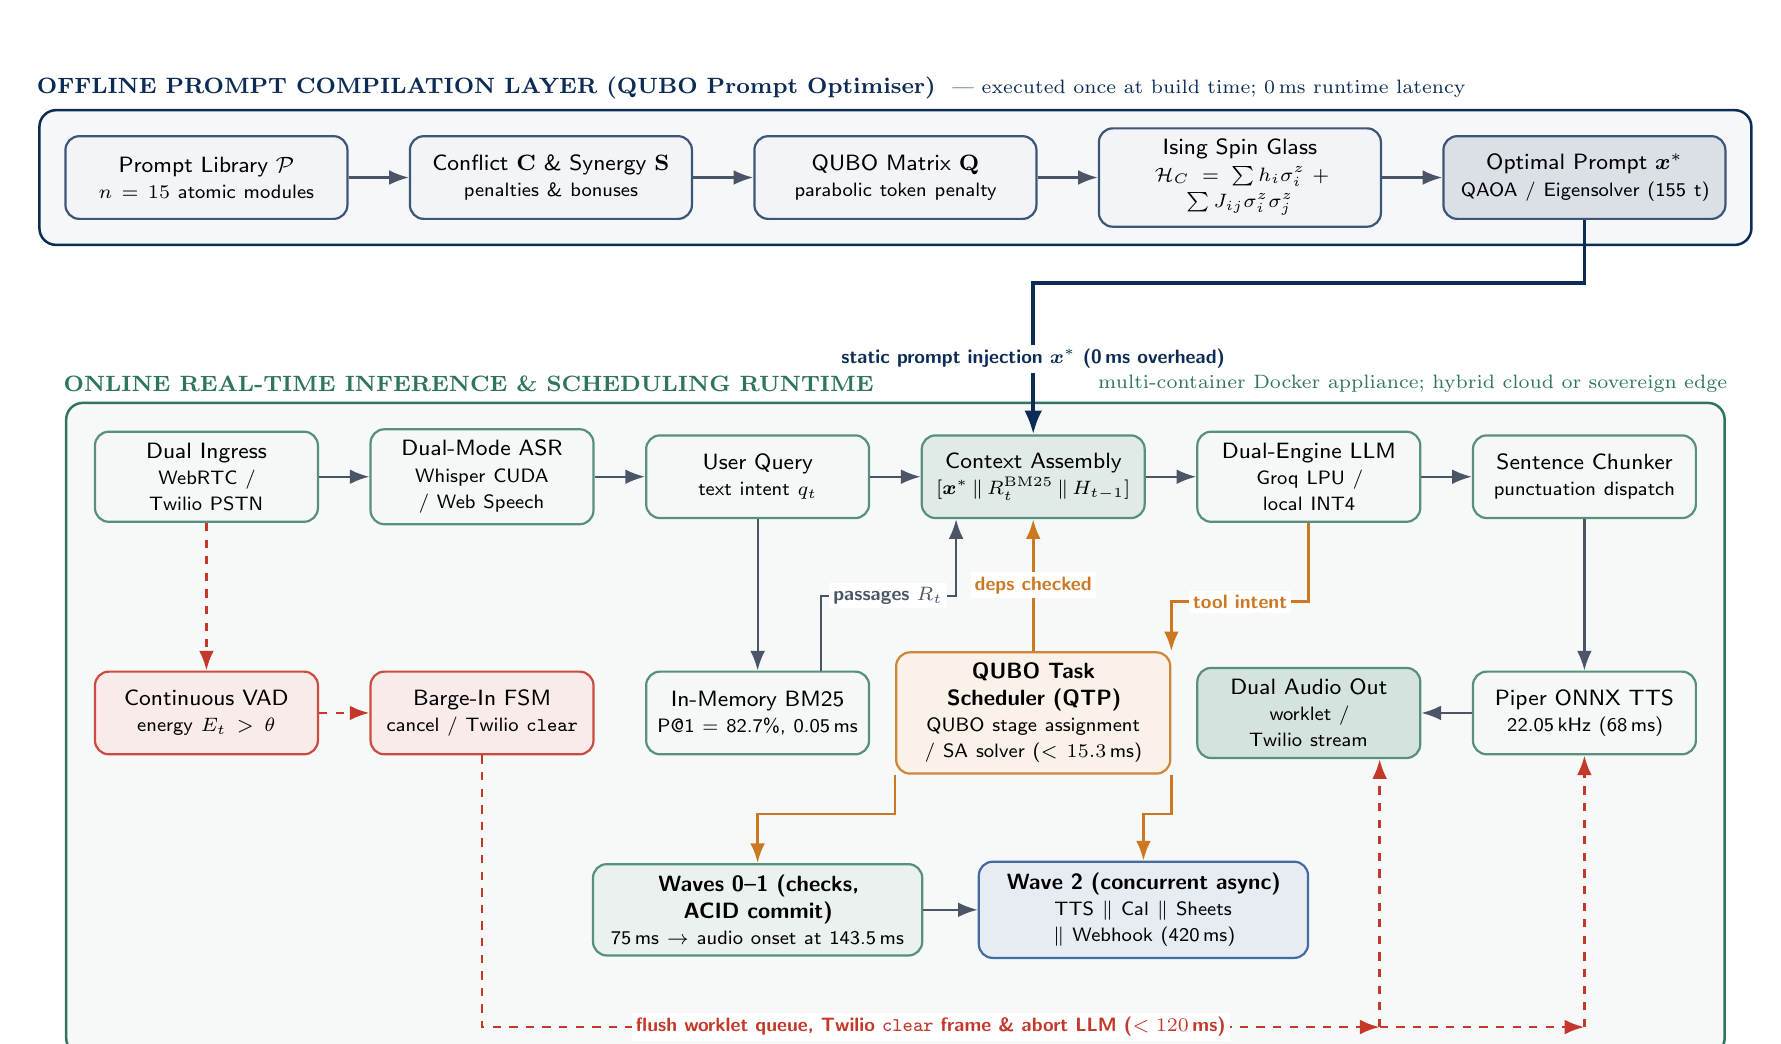
\begin{tikzpicture}[
  font=\sffamily\footnotesize,
  >=Latex,
  node distance=0pt,
  box/.style={rectangle, rounded corners=5pt, line width=0.8pt, align=center,
              inner sep=4pt, minimum height=1.05cm, text width=2.55cm},
  off/.style={box, draw=eaNavy!80, fill=eaNavy!5, text width=3.3cm},
  on/.style={box, draw=eaOlive!80, fill=eaOlive!5},
  barge/.style={box, draw=eaCoral!90, fill=eaCoral!10},
  qtp/.style={box, draw=eaAmber!90, fill=eaAmber!10, text width=3.2cm},
  wave/.style={box, draw=eaAmber!80, fill=white, text width=3.9cm, minimum height=1.0cm},
  arr/.style={-{Latex[length=2.5mm]}, line width=0.8pt, draw=eaSlate},
  arrNavy/.style={-{Latex[length=3mm]}, line width=1.3pt, draw=eaNavy},
  arrCoral/.style={-{Latex[length=2.5mm]}, line width=1.0pt, draw=eaCoral, dashed},
  arrAmber/.style={-{Latex[length=2.5mm]}, line width=1.0pt, draw=eaAmber},
  lbl/.style={font=\scriptsize\bfseries\sffamily, inner sep=1.5pt, fill=white, text opacity=1, anchor=center}
]

% ====================== OFFLINE LAYER (y = 13.4) ======================
\node[off] (pLib)   at (0,12.2)    {Prompt Library $\mathcal{P}$\\ {\scriptsize $n=15$ atomic modules}};
\node[off] (penMat) at (4.375,12.2)  {Conflict $\mathbf{C}$ \& Synergy $\mathbf{S}$\\ {\scriptsize penalties \& bonuses}};
\node[off] (qubo)   at (8.75,12.2)  {QUBO Matrix $\mathbf{Q}$\\ {\scriptsize parabolic token penalty}};
\node[off] (ising)  at (13.125,12.2) {Ising Spin Glass\\ {\scriptsize $\mathcal{H}_C=\sum h_i\sigma_i^z+\sum J_{ij}\sigma_i^z\sigma_j^z$}};
\node[off, fill=eaNavy!15] (opt) at (17.5,12.2) {Optimal Prompt $\bm{x}^*$\\ {\scriptsize QAOA / Eigensolver (155 t)}};

\draw[arr] (pLib)   -- (penMat);
\draw[arr] (penMat) -- (qubo);
\draw[arr] (qubo)   -- (ising);
\draw[arr] (ising)  -- (opt);

\begin{scope}[on background layer]
  \node[draw=eaNavy, fill=eaNavy!4, rounded corners=6pt, line width=0.9pt,
        inner sep=9pt, fit=(pLib)(opt), label={[font=\bfseries\footnotesize\color{eaNavy}, anchor=south west, xshift=-4pt]north west:%
        OFFLINE PROMPT COMPILATION LAYER (QUBO Prompt Optimiser) {\normalfont\scriptsize\ --- executed once at build time; 0\,ms runtime latency}}] (offBox) {};
\end{scope}

% ====================== ONLINE LAYER ======================
% Row 1 (y = 8.4): main streaming pipeline
\node[on] (audioIn) at (0,8.4)    {Dual Ingress\\ {\scriptsize WebRTC / Twilio PSTN}};
\node[on] (asr)     at (3.5,8.4)  {Dual-Mode ASR\\ {\scriptsize Whisper CUDA / Web Speech}};
\node[on] (query)   at (7.0,8.4)  {User Query\\ {\scriptsize text intent $q_t$}};
\node[on, fill=eaOlive!15] (ctx) at (10.5,8.4) {Context Assembly\\ {\scriptsize $[\bm{x}^*\,\|\,R_t^{\mathrm{BM25}}\,\|\,H_{t-1}]$}};
\node[on] (llm)     at (14.0,8.4) {Dual-Engine LLM\\ {\scriptsize Groq LPU / local INT4}};
\node[on] (chunk)   at (17.5,8.4) {Sentence Chunker\\ {\scriptsize punctuation dispatch}};

\draw[arr] (audioIn) -- (asr);
\draw[arr] (asr)     -- (query);
\draw[arr] (query)   -- (ctx);
\draw[arr] (ctx)     -- (llm);
\draw[arr] (llm)     -- (chunk);

% Row 2 (y = 5.2): VAD / barge-in / BM25 / QTP / audio out / TTS
\node[barge] (vad)  at (0,5.4)    {Continuous VAD\\ {\scriptsize energy $E_t>\theta$}};
\node[barge] (barge) at (3.5,5.4) {Barge-In FSM\\ {\scriptsize cancel / Twilio \texttt{clear}}};
\node[on]    (bm25) at (7.0,5.4)  {In-Memory BM25\\ {\scriptsize P@1 = 82.7\%, 0.05\,ms}};
\node[qtp]   (qtpN) at (10.5,5.4) {\textbf{QUBO Task Scheduler (QTP)}\\ {\scriptsize QUBO stage assignment / SA solver ($<15.3$\,ms)}};
\node[on, fill=eaOlive!20] (aout) at (14.0,5.4) {Dual Audio Out\\ {\scriptsize worklet / Twilio stream}};
\node[on]    (tts)  at (17.5,5.4) {Piper ONNX TTS\\ {\scriptsize 22.05\,kHz (68\,ms)}};

% Row 3 (y = 2.4): QTP waves
\node[wave, draw=eaOlive!80, fill=eaOlive!10] (w0) at (7.0,2.9)
  {\textbf{Waves 0--1 (checks, ACID commit)}\\ {\scriptsize 75\,ms $\to$ audio onset at 143.5\,ms}};
\node[wave, draw=eaNavy2!80, fill=eaNavy2!10] (w1) at (11.9,2.9)
  {\textbf{Wave 2 (concurrent async)}\\ {\scriptsize TTS $\parallel$ Cal $\parallel$ Sheets $\parallel$ Webhook (420\,ms)}};

% ---- Row 2 connections
\draw[arrCoral] (audioIn.south) -- (vad.north);
\draw[arrCoral] (vad.east) -- (barge.west);
\draw[arr] (query.south) -- (bm25.north);
\draw[arr] (chunk.south) -- (tts.north);
\draw[arr] (tts.west) -- (aout.east);

% BM25 -> Context Assembly (leaves BM25 top, runs in the row gutter, enters Context from below)
\draw[arr] ($(bm25.north)+(0.8,0)$) -- ++(0,0.95) coordinate (bmA) -| ($(ctx.south west)+(0.45,0)$);
\node[lbl, text=eaSlate] at ($(bmA)!0.5!(bmA -| ctx.south west)+(0.22,0)$) {passages $R_t$};

% LLM tool intent -> QTP
\draw[arrAmber] (llm.south) -- ++(0,-1.0) coordinate (ti) -| (qtpN.north east);
\node[lbl, text=eaAmber] at ($(ti)!0.5!(ti -| qtpN.north east)$) {tool intent};
% QTP -> Context (dependency-checked)
\draw[arrAmber] (qtpN.north) -- (ctx.south) node[lbl, text=eaAmber, midway] {deps checked};

% QTP -> waves
\draw[arrAmber] (qtpN.south west) -- ++(0,-0.5) -| (w0.north);
\draw[arrAmber] (qtpN.south east) -- ++(0,-0.5) -| (w1.north);
\draw[arr] (w0.east) -- (w1.west);

% Wave 0 eager TTS feeds audio out (via right of wave1 to keep gutter clear)
% Barge-in interrupt bus along the bottom (y = 0.6)
\draw[arrCoral] (barge.south) -- ++(0,-3.45) coordinate (bus1) -- (bus1 -| 14.9,0) coordinate (busA);
\draw[arrCoral] (busA) -- (busA |- aout.south);
\draw[arrCoral] (busA) -- (busA -| tts.south) coordinate (busB);
\draw[arrCoral] (busB) -- (tts.south);
\node[lbl, text=eaCoral] at ($(bus1)!0.5!(busA)$) {flush worklet queue, Twilio \texttt{clear} frame \& abort LLM ($<120$\,ms)};

% Static prompt injection (between layers)
\draw[arrNavy] (opt.south) -- ++(0,-0.8) coordinate (inj) -| (ctx.north);
\node[lbl, text=eaNavy] at ($(inj -| ctx.north)!0.5!(ctx.north)$) {static prompt injection $\bm{x}^*$ (0\,ms overhead)};

\begin{scope}[on background layer]
  \node[draw=eaOlive, fill=eaOlive!4, rounded corners=6pt, line width=0.9pt,
        inner sep=10pt, fit=(audioIn)(chunk)(vad)(tts)(w0)(w1)(bus1),
        label={[font=\bfseries\footnotesize\color{eaOlive}, anchor=south west, xshift=-4pt]north west:ONLINE REAL-TIME INFERENCE \& SCHEDULING RUNTIME},
        label={[font=\scriptsize\color{eaOlive}, anchor=south east, xshift=4pt]north east:multi-container Docker appliance; hybrid cloud or sovereign edge}] (onBox) {};
\end{scope}

\end{tikzpicture}
}%
\caption{Two-stage voice-agent architecture. The offline QPO layer selects a prompt configuration using QUBO/Ising optimization. The online pipeline combines speech recognition, lexical retrieval, streamed language-model output, speech synthesis, interruption handling, and QTP scheduling. QTP assigns dependent operations to execution waves; the $4.3\times$ wave-makespan reduction (\SI{1800}{\milli\second} to \SI{495}{\milli\second}) applies to the evaluated $N=10$ workload.}
\label{fig:architecture}
\end{figure*}

The evaluation covers two transaction domains: hospitality concierge tasks and clinical appointment triage. It uses 320 dialogue turns for voice-rule compliance and factual-detail retention, 300 logged dialogue turns for component-level latency measurements (60 of which were recorded with two-channel acoustic loopback for the percentile statistics of Table~\ref{tab:latency}), 100 telephone calls for telephony measurements, and 200 booking operations for synchronization reliability. 

\subsection{Data Preprocessing}
The runtime pipeline retrieves relevant passages from domain-specific knowledge bases and applies prompt directives governing Markdown suppression, concise responses, question limits, and factual grounding. 

\subsection{Model Development and System Architecture}
The following subsections detail the mathematical formulations, optimization procedures, voice pipeline architecture, interruption handling, enterprise integrations, and edge deployment topology. The framework uses two optimization stages: the offline QUBO Prompt Optimiser (QPO) compiles prompt directives, while the runtime QUBO Task Scheduler (QTP) schedules dependent tool operations.

\subsection{The QUBO Prompt Optimiser (QPO) Formulation}
Let $\mathcal{P} = \{P_1, P_2, \ldots, P_n\}$ denote a library of $n$ atomic candidate prompt directives. Each directive $P_i$ represents a self-contained behavioral instruction and belongs to one of the following categories:
\begin{equation}
  \mathcal{P} = \mathcal{P}_{\mathrm{persona}} \cup \mathcal{P}_{\mathrm{tone}} \cup \mathcal{P}_{\mathrm{rule}} \cup \mathcal{P}_{\mathrm{guardrail}} \cup \mathcal{P}_{\mathrm{rag}} \cup \mathcal{P}_{\mathrm{action}}
\end{equation}
Each instruction $P_i$ is characterized by two coefficients: its token cost $t_i \in \mathbb{N}^+$, which represents the number of tokens it adds to the LLM context, and its baseline semantic utility $v_i \in \mathbb{R}^+$, which represents its estimated contribution to conversational quality.

A prompt configuration is represented by an $n$-dimensional binary decision vector:
\begin{equation}
  \bm{x} = [x_1, x_2, \ldots, x_n]^T \in \{0, 1\}^n
\end{equation}
Here, $x_i = 1$ indicates that directive $P_i$ is included in the system prompt, whereas $x_i = 0$ indicates that it is excluded.

Directives cannot be selected independently because they interact in several ways:
\begin{enumerate}[noitemsep]
  \item \textbf{Pairwise Directive Conflicts}: A symmetric, non-negative conflict matrix $\mathbf{C} \in \mathbb{R}_{\ge 0}^{n \times n}$ assigns a penalty when directives $P_i$ and $P_j$ are selected together ($x_i x_j = 1$). A positive value of $C_{ij}$ indicates that the directives are mutually exclusive or logically incompatible, such as a terse response requirement paired with a highly detailed explanatory persona.
  \item \textbf{Acoustic and Semantic Synergy}: A symmetric, non-negative synergy matrix $\mathbf{S} \in \mathbb{R}_{\ge 0}^{n \times n}$ assigns a reward to pairs of directives that provide a combined benefit when selected together. For example, combining a brevity constraint with Markdown suppression may reduce formatting artifacts in speech output and lower token-generation overhead.
  \item \textbf{Quadratic Token-Budget Penalty}: The total prompt length is $\sum_{i=1}^n t_i x_i = \bm{t}^T \bm{x}$. To encourage the selected directives to remain close to a target token budget $T \in \mathbb{N}^+$, while penalizing both underuse and overuse of the budget, we define the quadratic deviation penalty:
  \begin{equation}
    \Phi(\bm{x}) = \left(\sum_{i=1}^n t_i x_i - T\right)^2 = \left(\bm{t}^T \bm{x} - T\right)^2
    \label{eq:budget_penalty}
  \end{equation}
  The optimization in Eq.~\eqref{eq:primal_objective} uses the normalized form of this penalty ($\tau_i = t_i/T$) so that it remains commensurate with the utilities $v_i$.
\end{enumerate}

\begin{table}[t]
\centering
\small
\setlength{\tabcolsep}{3.5pt}
\renewcommand{\arraystretch}{1.12}
\caption{Mathematical notation and operational definitions for the QUBO Prompt Optimiser (QPO) and QUBO Task Scheduler (QTP).}
\label{tab:notation}
\begin{tabularx}{\columnwidth}{|l|X|}
\hline
\textbf{Symbol} & \textbf{Operational Definition} \\
\hline
$\mathcal{P}, n$ & Prompt module library and cardinality ($n=15$) \\
\hline
$\bm{x} \in \{0, 1\}^n$ & Binary decision vector of module selection \\
\hline
$t_i, v_i$ & Token consumption cost and semantic value of module $P_i$ \\
\hline
$\mathbf{C}, \mathbf{S} \in \mathbb{R}^{n \times n}$ & Pairwise conflict penalty and synergy reward matrices \\
\hline
$T, \mu$ & Target token budget ($T=150$) and penalty weight ($\mu \in [16, 64]$) \\
\hline
$\mathbf{Q} \in \mathbb{R}^{n \times n}$ & Upper-triangular QUBO interaction matrix \\
\hline
$\mathcal{H}_C, \mathcal{H}_M$ & Problem cost and transverse mixer Hamiltonians \\
\hline
$\sigma_i^z, \sigma_i^x$ & Pauli spin-1/2 operators on the $i$-th qubit \\
\hline
$\bm{z} \in \{-1, +1\}^n$ & Ising spin configuration vector ($z_i = 1 - 2x_i$) \\
\hline
$p, (\bm{\gamma}, \bm{\beta})$ & QAOA circuit depth and variational parameter vectors \\
\hline
$E_t, \theta, C_{\mathrm{th}}$ & RMS frame energy, barge-in threshold, and hysteresis limit \\
\hline
\hline
\end{tabularx}\end{table}

\subsection{Derivation of the Upper-Triangular QUBO Matrix}
The aim of the QUBO Prompt Optimiser is to maximize composite conversational fitness while minimizing budget deviation, directive conflicts, and persona inconsistency. Following standard quadratic encodings for constrained binary optimization~\citep{Glover2019}, we define normalized token proportions $\tau_i = t_i / T$ with respect to target budget $T$. Incorporating regularization weight $\mu \in [16, 64]$ and an exclusivity constraint (enforced by a penalty) over the persona index set $\mathcal{P}_{\mathrm{persona}} = \{1, 2\}$ with penalty weight $\lambda = 5.0$, the primal objective is formulated as:
\begin{equation}
  \max_{\bm{x} \in \{0, 1\}^n} \left[ \sum_{i=1}^n v_i x_i - \sum_{i < j} C_{ij} x_i x_j + \sum_{i < j} S_{ij} x_i x_j - \mu \left(\sum_{i=1}^n \tau_i x_i - 1\right)^2 - \lambda \left(\sum_{a \in \mathcal{P}_{\mathrm{persona}}} x_a - 1\right)^2 \right]
  \label{eq:primal_objective}
\end{equation}
Normalizing token footprints by $T$ keeps the budget regularization commensurate with the semantic utilities ($v_i \in [0, 1]$), avoiding the unnormalized token terms that would otherwise dominate the objective.

In combinatorial optimization, Quadratic Unconstrained Binary Optimization is canonically stated as a minimization problem:
\begin{equation}
  \min_{\bm{x} \in \{0, 1\}^n} \mathcal{F}(\bm{x}) = \bm{x}^T \mathbf{Q} \bm{x} + \mathrm{const}
  \label{eq:qubo_canonical}
\end{equation}
where $\mathbf{Q} \in \mathbb{R}^{n \times n}$ is an upper-triangular matrix.

\begin{theorem}[QUBO Matrix Representation]
The prompt optimization objective in Eq.~\eqref{eq:primal_objective} is equal to minimizing the canonical quadratic form in Eq.~\eqref{eq:qubo_canonical}, where the elements of $\mathbf{Q}$ are given by:
\begin{align}
  Q_{ii} &= -v_i + \mu \left(\tau_i^2 - 2 \tau_i\right) - \lambda \cdot \mathbb{I}(i \in \mathcal{P}_{\mathrm{persona}}) \quad \forall i \in \{1, \ldots, n\} \label{eq:q_diag} \\
  Q_{ij} &= C_{ij} - S_{ij} + 2 \mu \tau_i \tau_j + 2\lambda \cdot \mathbb{I}(i, j \in \mathcal{P}_{\mathrm{persona}}) \quad \forall i < j \label{eq:q_offdiag}
\end{align}
\end{theorem}

\begin{proof}
Negating the maximization objective in Eq.~\eqref{eq:primal_objective} yields the equivalent minimization task:
\begin{align}
  \mathcal{F}(\bm{x}) &= -\sum_{i=1}^n v_i x_i + \sum_{i < j} C_{ij} x_i x_j - \sum_{i < j} S_{ij} x_i x_j \nonumber \\
  &\quad + \mu \left(\sum_{i=1}^n \tau_i x_i - 1\right)^2 + \lambda \left(\sum_{a \in \mathcal{P}_{\mathrm{persona}}} x_a - 1\right)^2
\end{align}
Expanding the normalized quadratic budget penalty:
\begin{align}
  \left(\sum_{i=1}^n \tau_i x_i - 1\right)^2 &= \left(\sum_{i=1}^n \tau_i x_i\right)^2 - 2 \sum_{i=1}^n \tau_i x_i + 1 \nonumber \\
  &= \sum_{i=1}^n \tau_i^2 x_i^2 + 2 \sum_{i < j} \tau_i \tau_j x_i x_j - 2 \sum_{i=1}^n \tau_i x_i + 1
\end{align}
Exploiting binary idempotency $x_i^2 = x_i$:
\begin{align}
  \left(\sum_{i=1}^n \tau_i x_i - 1\right)^2 &= \sum_{i=1}^n (\tau_i^2 - 2 \tau_i) x_i + \sum_{i < j} 2 \tau_i \tau_j x_i x_j + 1
\end{align}
Similarly, expanding the persona constraint:
\begin{align}
  \left(\sum_{a \in \mathcal{P}_{\mathrm{persona}}} x_a - 1\right)^2 &= \sum_{a} (-x_a) + 2 \sum_{a < b} x_a x_b + 1
\end{align}
Substituting both expansions into the minimization function and collecting linear ($x_i$) and bilinear ($x_i x_j$) terms establishes Eqs.~\eqref{eq:q_diag} and~\eqref{eq:q_offdiag}, where constant scalar offsets do not affect the argmin location.
\end{proof}

\begin{figure}[t]
\centering
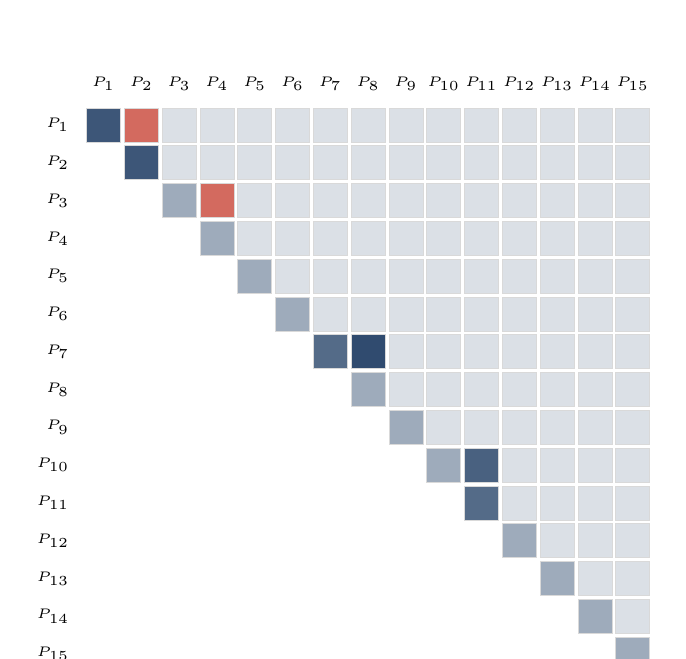
\begin{tikzpicture}[scale=0.48, every node/.style={font=\sffamily\tiny}]
  % 15x15 Matrix Heatmap
  \foreach \i in {1,...,15} {
    \foreach \j in {\i,...,15} {
      \pgfmathsetmacro{\val}{
        ifthenelse(\i == \j,
          (\i==1|| \i==2 ? 0.8 : (\i==7 || \i==11 ? 0.7 : 0.4)),
          ((\i==1 && \j==2) ? -0.9 :
          ((\i==3 && \j==4) ? -0.6 :
          ((\i==7 && \j==8) ? 0.85 :
          ((\i==10 && \j==11) ? 0.75 : 0.15))))
        )
      }
      \pgfmathparse{\val < 0 ? 1 : 0}
      \ifnum\pgfmathresult=1
        \pgfmathsetmacro{\cval}{-\val*100}
        \definecolor{cellcol}{RGB}{196,56,42}
        \fill[cellcol, fill opacity=0.75] (\j-1, 15-\i) rectangle ++(0.9, 0.9);
      \else
        \pgfmathsetmacro{\cval}{\val*100}
        \definecolor{cellcol}{RGB}{12,44,86}
        \fill[cellcol, fill opacity=\val] (\j-1, 15-\i) rectangle ++(0.9, 0.9);
      \fi
      \draw[gray!30, line width=0.2pt] (\j-1, 15-\i) rectangle ++(0.9, 0.9);
    }
    % Label on left
    \node[anchor=east] at (-0.2, 15.45-\i) {$P_{\i}$};
    % Label on top
    \node[anchor=south] at (\i-0.55, 15.1) {$P_{\i}$};
  }
\end{tikzpicture}
\caption{Schematic visualization (cell shading illustrative, not to scale) of the upper-triangular QUBO interaction matrix $\mathbf{Q} \in \mathbb{R}^{15 \times 15}$ compiled for the hospitality concierge domain ($T=150$, $\mu=64.0$, $\lambda=5.0$). Blue cells denote attractive terms (diagonal utility and synergistic co-occurrence bonuses); coral cells indicate conflict penalties ($C_{1,2} = 1.0$, $C_{3,4} = 0.45$).}
\label{fig:qubo_matrix}
\end{figure}

\subsection{Bijection to the Ising Spin Glass Hamiltonian}
To express the objective as an Ising Hamiltonian, binary variables $x_i \in \{0, 1\}$ are mapped to spin variables $z_i \in \{-1, +1\}$ via the standard affine transformation~\citep{Lucas2014}; this yields an equivalent problem, not a speedup:
\begin{equation}
  x_i = \frac{1 - z_i}{2} \iff z_i = 1 - 2x_i
  \label{eq:spin_transform}
\end{equation}
Under this mapping, $z_i = -1$ corresponds to $x_i = 1$, while $z_i = +1$ corresponds to $x_i = 0$.

In the quantum formulation, the spin variables are represented by Pauli-$z$ operators $\sigma_i^z = \left(\begin{smallmatrix} 1 & 0 \\ 0 & -1 \end{smallmatrix}\right)$ acting on the Hilbert space $\mathcal{H} = (\mathbb{C}^2)^{\otimes n}$.

\begin{theorem}[Ising Cost Hamiltonian Mapping]
The QUBO prompt optimization problem maps identically to finding the ground-state of an Ising spin glass Hamiltonian with longitudinal magnetic fields $h_i$ and two-body exchange couplings $J_{ij}$:
\begin{equation}
  \mathcal{H}_C = \sum_{i=1}^n h_i \sigma_i^z + \sum_{i < j} J_{ij} \sigma_i^z \sigma_j^z + \mathcal{E}_0 \mathbf{I}
  \label{eq:ising_hamiltonian}
\end{equation}
The corresponding coefficients are:
\begin{align}
  h_i &= -\frac{1}{2} Q_{ii} - \frac{1}{4} \sum_{j < i} Q_{ji} - \frac{1}{4} \sum_{j > i} Q_{ij} \label{eq:h_field} \\
  J_{ij} &= \frac{1}{4} Q_{ij} \quad \forall i < j \label{eq:j_coupling} \\
  \mathcal{E}_0 &= \frac{1}{2} \sum_{i=1}^n Q_{ii} + \frac{1}{4} \sum_{i < j} Q_{ij} \label{eq:e_offset}
\end{align}
\end{theorem}

\begin{proof}
Substituting the transformation $x_i = \frac{1 - \sigma_i^z}{2}$ into the canonical QUBO form:
\begin{align}
  \bm{x}^T \mathbf{Q} \bm{x} &= \sum_{i=1}^n Q_{ii} \left(\frac{\mathbf{I} - \sigma_i^z}{2}\right) + \sum_{i < j} Q_{ij} \left(\frac{\mathbf{I} - \sigma_i^z}{2}\right)\left(\frac{\mathbf{I} - \sigma_j^z}{2}\right) \nonumber \\
  &= \frac{1}{2}\sum_{i=1}^n Q_{ii}(\mathbf{I} - \sigma_i^z) + \frac{1}{4}\sum_{i < j} Q_{ij}(\mathbf{I} - \sigma_i^z - \sigma_j^z + \sigma_i^z \sigma_j^z)
\end{align}
Regrouping terms by operator rank:
\begin{align}
  \bm{x}^T \mathbf{Q} \bm{x} &= \underbrace{\left[\frac{1}{2}\sum_{i=1}^n Q_{ii} + \frac{1}{4}\sum_{i < j} Q_{ij}\right]}_{\mathcal{E}_0} \mathbf{I} \nonumber \\
  &\quad + \sum_{i=1}^n \underbrace{\left[-\frac{1}{2}Q_{ii} - \frac{1}{4}\sum_{j < i} Q_{ji} - \frac{1}{4}\sum_{j > i} Q_{ij}\right]}_{h_i} \sigma_i^z \nonumber \\
  &\quad + \sum_{i < j} \underbrace{\left[\frac{1}{4}Q_{ij}\right]}_{J_{ij}} \sigma_i^z \sigma_j^z
\end{align}
This expansion matches Eq.~\eqref{eq:ising_hamiltonian} exactly.
\end{proof}

\subsection{Quantum Approximate Optimization Algorithm (QAOA)}
To approximate the ground state $|\psi_{\mathrm{opt}}\rangle$, which satisfies $\mathcal{H}_C |\psi_{\mathrm{opt}}\rangle = E_{\min} |\psi_{\mathrm{opt}}\rangle$, we use the Quantum Approximate Optimization Algorithm (QAOA) as described and analyzed by \citet{Zhou2020}, with the generalized ansatz of \citet{Hadfield2019} as background. All QAOA runs reported here are statevector simulations. The algorithm constructs a parameterized trial state by applying $p$ alternating unitary operators to an initial uniform superposition state:
\begin{equation}
  |+\rangle^{\otimes n} = \frac{1}{\sqrt{2^n}} \sum_{\bm{z} \in \{-1, 1\}^n} |\bm{z}\rangle
\end{equation}
The depth-$p$ ansatz state is built as:
\begin{equation}
  |\bm{\gamma}, \bm{\beta}\rangle = \prod_{k=1}^p \mathcal{U}_M(\beta_k) \mathcal{U}_C(\gamma_k) |+\rangle^{\otimes n}
\end{equation}
where $\mathcal{U}_C(\gamma) = \exp(-i \gamma \mathcal{H}_C)$ is the cost unitary and $\mathcal{U}_M(\beta) = \exp(-i \beta \mathcal{H}_M)$ is the transverse-field mixer unitary, with:
\begin{equation}
  \mathcal{H}_M = -\sum_{i=1}^n \sigma_i^x
\end{equation}

\begin{algorithm}[t]
\caption{Offline Prompt Optimization via QAOA / Ising Eigensolver}
\label{alg:qaoa_compilation}
\begin{algorithmic}[1]
\Require Directive library $\mathcal{P}$, values $\bm{v}$, normalized lengths $\bm{\tau} = \bm{t}/T$, penalty $\mathbf{C}$, synergy $\mathbf{S}$, weights $\mu, \lambda$, persona set $\mathcal{P}_{\mathrm{persona}}$, depth $p$.
\Ensure Optimal binary prompt configuration $\bm{x}^* \in \{0, 1\}^n$.
\State Compute $Q_{ii} \leftarrow -v_i + \mu(\tau_i^2 - 2\tau_i) - \lambda \cdot \mathbb{I}(i \in \mathcal{P}_{\mathrm{persona}})$ for all $i \in \{1, \ldots, n\}$;
\State Compute $Q_{ij} \leftarrow C_{ij} - S_{ij} + 2\mu \tau_i \tau_j + 2\lambda \cdot \mathbb{I}(i, j \in \mathcal{P}_{\mathrm{persona}})$ for all $i < j$;
\State Compute fields $h_i$ and couplings $J_{ij}$ via Eqs.~\eqref{eq:h_field}--\eqref{eq:j_coupling};
\State Construct cost Hamiltonian $\mathcal{H}_C = \sum h_i \sigma_i^z + \sum J_{ij}\sigma_i^z\sigma_j^z$;
\State Initialize state $|+\rangle^{\otimes n} = \frac{1}{\sqrt{2^n}}\sum_{\bm{z} \in \{-1, 1\}^n} |\bm{z}\rangle$;
\State Set initial variational parameters $(\bm{\gamma}^{(0)}, \bm{\beta}^{(0)}) \in [0, 2\pi]^p \times [0, \pi]^p$;
\For{iteration $k = 1, 2, \ldots, K_{\max}$}
  \State Construct state $|\bm{\gamma}^{(k)}, \bm{\beta}^{(k)}\rangle = \prod_{l=1}^p e^{-i \beta_l \mathcal{H}_M} e^{-i \gamma_l \mathcal{H}_C} |+\rangle^{\otimes n}$;
  \State Evaluate energy expectation $\langle E \rangle = \langle \bm{\gamma}^{(k)}, \bm{\beta}^{(k)} | \mathcal{H}_C | \bm{\gamma}^{(k)}, \bm{\beta}^{(k)} \rangle$;
  \State Update $(\bm{\gamma}^{(k+1)}, \bm{\beta}^{(k+1)}) \leftarrow \mathrm{COBYLA}(\langle E \rangle, \bm{\gamma}^{(k)}, \bm{\beta}^{(k)})$;
  \If{$|\langle E \rangle^{(k)} - \langle E \rangle^{(k-1)}| < \epsilon$}
    \State \textbf{break};
  \EndIf
\EndFor
\State Sample bitstrings $\bm{z} \sim |\langle \bm{z} | \bm{\gamma}^*, \bm{\beta}^* \rangle|^2$ for $N_{\mathrm{shots}} = 256$ shots;
\State $\bm{z}^* \leftarrow \arg\min_{\bm{z}} \langle \bm{z} | \mathcal{H}_C | \bm{z} \rangle$;
\State \Return $\bm{x}^* = \frac{1}{2}(\mathbf{1} - \bm{z}^*)$.
\end{algorithmic}
\end{algorithm}

\begin{figure}[t]
\centering
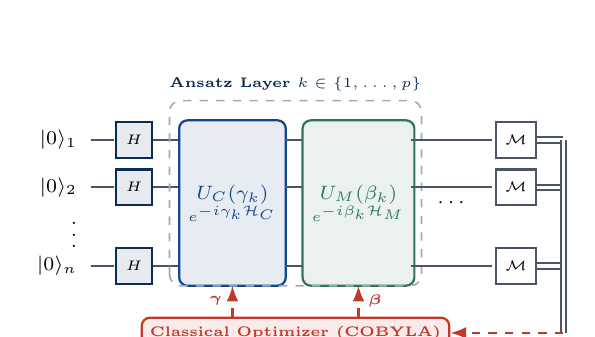
\begin{tikzpicture}[
  font=\sffamily\scriptsize,
  wire/.style={line width=0.7pt, draw=eaSlate},
  clwire/.style={line width=0.7pt, draw=eaSlate, double, double distance=1.2pt},
  gate/.style={rectangle, draw=eaNavy, fill=eaNavy!10, line width=0.8pt, minimum size=0.45cm, align=center, font=\tiny\bfseries},
  blockU/.style={rectangle, draw=eaNavy2, fill=eaNavy2!10, rounded corners=3pt, line width=0.8pt, minimum width=1.35cm, minimum height=2.1cm, align=center, font=\scriptsize\bfseries\color{eaNavy2}},
  blockM/.style={rectangle, draw=eaOlive, fill=eaOlive!10, rounded corners=3pt, line width=0.8pt, minimum width=1.35cm, minimum height=2.1cm, align=center, font=\scriptsize\bfseries\color{eaOlive}},
  meas/.style={rectangle, draw=eaSlate, fill=white, line width=0.8pt, minimum size=0.45cm, align=center, font=\tiny\bfseries}
]
  % Input state labels
  \node[anchor=east, font=\scriptsize] at (0, 1.8) {$|0\rangle_1$};
  \node[anchor=east, font=\scriptsize] at (0, 1.2) {$|0\rangle_2$};
  \node[anchor=east, font=\scriptsize] at (0, 0.7) {$\vdots$};
  \node[anchor=east, font=\scriptsize] at (0, 0.2) {$|0\rangle_n$};

  % Quantum wires before layer
  \draw[wire] (0.05, 1.8) -- (0.35, 1.8);
  \draw[wire] (0.05, 1.2) -- (0.35, 1.2);
  \draw[wire] (0.05, 0.2) -- (0.35, 0.2);

  % Hadamard gates
  \node[gate] (h1) at (0.6, 1.8) {$H$};
  \node[gate] (h2) at (0.6, 1.2) {$H$};
  \node[gate] (hn) at (0.6, 0.2) {$H$};

  % Wires into Unitary blocks
  \draw[wire] (h1.east) -- (1.18, 1.8);
  \draw[wire] (h2.east) -- (1.18, 1.2);
  \draw[wire] (hn.east) -- (1.18, 0.2);

  % Unitary blocks
  \node[blockU] (uC) at (1.85, 1.0) {$U_C(\gamma_k)$\\ \normalfont\tiny $e^{-i\gamma_k \mathcal{H}_C}$};
  
  \draw[wire] (2.52, 1.8) -- (2.78, 1.8);
  \draw[wire] (2.52, 1.2) -- (2.78, 1.2);
  \draw[wire] (2.52, 0.2) -- (2.78, 0.2);

  \node[blockM] (uM) at (3.45, 1.0) {$U_M(\beta_k)$\\ \normalfont\tiny $e^{-i\beta_k \mathcal{H}_M}$};

  % Layer bounding bracket
  \draw[draw=eaNavy!40, dashed, rounded corners=4pt, line width=0.6pt] 
    (1.05, -0.05) rectangle (4.25, 2.3);
  \node[anchor=south, font=\tiny\bfseries\color{eaNavy}] at (2.65, 2.3) {Ansatz Layer $k \in \{1,\dots,p\}$};

  % Wires to measurement
  \draw[wire] (4.12, 1.8) -- (5.15, 1.8);
  \draw[wire] (4.12, 1.2) -- (5.15, 1.2);
  \draw[wire] (4.12, 0.2) -- (5.15, 0.2);
  \node[fill=white, inner sep=2pt, font=\scriptsize\bfseries] at (4.65, 1.0) {$\cdots$};

  % Measurement gates
  \node[meas] (m1) at (5.45, 1.8) {$\mathcal{M}$};
  \node[meas] (m2) at (5.45, 1.2) {$\mathcal{M}$};
  \node[meas] (mn) at (5.45, 0.2) {$\mathcal{M}$};

  % Classical measurement output lines
  \draw[clwire] (m1.east) -- (6.05, 1.8);
  \draw[clwire] (m2.east) -- (6.05, 1.2);
  \draw[clwire] (mn.east) -- (6.05, 0.2);
  \draw[clwire] (6.05, 1.8) -- (6.05, -0.65);

  % Classical Optimizer Block
  \node[draw=eaCoral, fill=eaCoral!10, rounded corners=3pt, line width=0.8pt, font=\tiny\bfseries\color{eaCoral}, inner sep=3pt] 
    (cobyla) at (2.65, -0.65) {Classical Optimizer (COBYLA)};

  \draw[-{Latex[length=2mm]}, line width=0.8pt, draw=eaCoral, dashed] 
    (6.05, -0.65) -- (cobyla.east);
  \draw[-{Latex[length=2mm]}, line width=0.8pt, draw=eaCoral, dashed] 
    (cobyla.north -| 1.85, 0) -- node[left, font=\tiny\color{eaCoral}] {$\bm{\gamma}$} (1.85, -0.05);
  \draw[-{Latex[length=2mm]}, line width=0.8pt, draw=eaCoral, dashed] 
    (cobyla.north -| 3.45, 0) -- node[right, font=\tiny\color{eaCoral}] {$\bm{\beta}$} (3.45, -0.05);
\end{tikzpicture}
\caption{QAOA parameterized quantum circuit ansatz. An initial uniform superposition state $|+\rangle^{\otimes n}$ undergoes $p$ alternating layers of problem cost unitary $U_C(\gamma)$ and transverse mixer unitary $U_M(\beta)$, followed by computational basis measurement and classical feedback optimization via a gradient-free optimizer such as COBYLA or SPSA.}
\label{fig:qaoa_convergence}
\end{figure}

\subsection{The QUBO Task Scheduler (QTP) for Runtime Concurrency Scheduling}
\label{sec:qtp_formulation}
The offline QPO layer optimizes prompt selection. During live dialogue, however, external state changes (such as booking a room, checking physician calendars, or sending notifications) introduce a separate bottleneck: the latency associated with executing multiple tasks. Stage assignment with precedence constraints is encoded as a QUBO following the penalty approach of \citet{Glover2019}; related QUBO models exist for job-shop scheduling~\citep{Geitz2022,Aggoune2023}, and dependency-graph execution of LLM function calls is studied by \citet{Kim2024}. 

In an enterprise transaction, a turn may involve a set of $N$ tasks, $\mathcal{T} = \{T_1, T_2, \dots, T_N\}$. Each task $T_i$ has an estimated duration $d_i > 0$, an execution type (blocking in-memory work or asynchronous network I/O), and a set of causal dependencies represented by a directed acyclic graph (DAG), $\mathcal{G}_{\text{prec}} = (\mathcal{T}, \mathcal{E}_{\text{prec}})$. An edge $(T_i, T_j) \in \mathcal{E}_{\text{prec}}$ indicates that task $T_i$ must finish before task $T_j$ can begin. If scheduled serially, the total execution makespan scales as:
\begin{equation}
M_{\text{serial}} = \sum_{i=1}^N d_i.
\end{equation}
For the $N=10$ booking workload of Table~\ref{tab:task_dag}, the serial makespan is \SI{1800}{\milli\second}. Under wave concurrency where tasks within wave $W_k$ run in parallel, the makespan is given by the sum of wave critical paths:
\begin{equation}
M_{\text{wave}} = \sum_{k=0}^{K-1} \max_{i \in W_k} d_i.
\end{equation}
Because remote synchronization depends only on the local SQLite commit, Wave~0 executes local validation ($T_1, T_2$), Wave~1 commits the ACID transaction ($T_3$), and Wave~2 executes audio synthesis ($T_4$) concurrently with remote synchronization and logging ($T_5$--$T_{10}$), yielding $M_{\text{wave}} = \max(25, 35) + 40 + \max(68.5, 312.4, 285.0, 195.0, 420.0, 65.0, 354.1) = \SI{495}{\milli\second}$ ($4.3\times$ speedup). Speech onset begins \SI{143.5}{\milli\second} after dispatch ($35 + 40 + 68.5\,\text{ms}$), masking background synchronization.

To reduce this delay while preserving transactional safety, we formulate task scheduling as a Quadratic Unconstrained Binary Optimization (QUBO) problem over discrete execution-stage assignments. Let $K$ denote the number of available stages (or waves), with $K \in \{2, 3\}$. We define the following binary decision variables:
\begin{equation}
y_{ik} \in \{0, 1\}, \quad \forall i \in \{1, \dots, N\}, \; k \in \{0, \dots, K-1\},
\end{equation}
where $y_{ik} = 1$ if task $T_i$ is assigned to stage $k$, and $y_{ik} = 0$ otherwise. The total number of binary variables, and hence the number of qubits in the corresponding formulation, is $\mathcal{N}_q = N \times K$.

The QTP objective combines four terms:
\begin{enumerate}[leftmargin=*]
  \item \textbf{One-Hot Stage Assignment}: Each task must be assigned to exactly one execution stage:
  \begin{equation}
  \mathcal{H}_{\text{one-hot}} = \sum_{i=1}^N \left( \sum_{k=0}^{K-1} y_{ik} - 1 \right)^2.
  \end{equation}
  \item \textbf{Precedence Constraints}: If task $T_i$ must precede task $T_j$, then $T_i$ cannot be assigned to the same stage as, or a later stage than, $T_j$:
  \begin{equation}
  \mathcal{H}_{\text{prec}} = \sum_{(T_i, T_j) \in \mathcal{E}_{\text{prec}}} \sum_{k=0}^{K-1} \sum_{k'=0}^k y_{ik} y_{jk'}.
  \end{equation}
  \item \textbf{Stage-Index Cost}: To encourage tasks to be assigned to earlier stages, each stage is assigned a weight $w_k = (k+1)$, and durations are normalized by the serial makespan so that the stage cost stays small relative to the constraint penalties below:
  \begin{equation}
  \mathcal{H}_{\text{stage}} = \sum_{k=0}^{K-1} \sum_{i=1}^N w_k \tilde{d}_i y_{ik}, \qquad \tilde{d}_i = d_i / M_{\text{serial}}.
  \end{equation}
  \item \textbf{Concurrency Synergy}: When compatible I/O-bound tasks, such as HTTP requests to Google Calendar and Google Sheets, run in the same stage $k$, their network operations can proceed concurrently. The formulation represents this benefit using a synergy coefficient $S_{ij} > 0$:
  \begin{equation}
  \mathcal{H}_{\text{synergy}} = \sum_{k=0}^{K-1} \sum_{1 \le i < j \le N} S_{ij} y_{ik} y_{jk}.
  \end{equation}
\end{enumerate}

The stage-index cost is a scheduling proxy, not an exact makespan expression; the realized makespan must be calculated from the scheduled task durations and precedence graph. The composite QTP Hamiltonian is defined as:
\begin{equation}
\label{eq:qtp_hamiltonian}
\mathcal{H}_{\text{QTP}} = \lambda_{\text{span}} \mathcal{H}_{\text{stage}} + \lambda_{\text{prec}} \mathcal{H}_{\text{prec}} + \lambda_{\text{one}} \mathcal{H}_{\text{one-hot}} - \lambda_{\text{syn}} \mathcal{H}_{\text{synergy}},
\end{equation}
where penalty coefficients $\lambda_{\text{one}} = 50.0$, $\lambda_{\text{prec}} = 40.0$, $\lambda_{\text{span}} = 1.0$, and $\lambda_{\text{syn}} = 2.0$ are chosen to exceed any achievable gain in the normalized stage cost (at most $K$), so that constraint violations are never favorable.

\begin{algorithm}[t]
\caption{Quantum Task Parallelization (QTP) Live Scheduling}
\label{alg:qtp}
\begin{algorithmic}[1]
\Require Task set $\mathcal{T} = \{T_1, \dots, T_N\}$, durations $\{d_i\}$, dependency DAG $\mathcal{E}_{\text{prec}}$, stage count $K$.
\Ensure Optimized stage dispatch plan $\mathcal{W} = \{W_0, \dots, W_{K-1}\}$.
\State Initialize upper-triangular QUBO matrix $\mathbf{Q}_{\text{QTP}} \in \mathbb{R}^{\mathcal{N}_q \times \mathcal{N}_q}$ with zeros.
\For{each task $i \in \{1, \dots, N\}$}
  \State Add one-hot penalty $\lambda_{\text{one}} (\sum_k y_{ik} - 1)^2$ to $\mathbf{Q}_{\text{QTP}}$.
  \For{each stage $k \in \{0, \dots, K-1\}$}
    \State $\mathbf{Q}_{\text{QTP}}[(i,k),(i,k)] \mathrel{+}= \lambda_{\text{span}} (k+1) \tilde{d}_i$.
  \EndFor
\EndFor
\For{each dependency $(T_i, T_j) \in \mathcal{E}_{\text{prec}}$}
  \For{$k=0$ to $K-1$}
    \For{$k'=0$ to $k$}
      \State $\mathbf{Q}_{\text{QTP}}[(i,k),(j,k')] \mathrel{+}= \lambda_{\text{prec}}$.
    \EndFor
  \EndFor
\EndFor
\For{each compatible concurrency pair $(i,j)$ and stage $k$}
  \State Add reward term $-\lambda_{\text{syn}} S_{ij} y_{ik}y_{jk}$ to $\mathbf{Q}_{\text{QTP}}$.
\EndFor
\State Solve ground state $\bm{y}^* = \arg\min_{\bm{y}} \bm{y}^T \mathbf{Q}_{\text{QTP}} \bm{y}$ via Simulated Annealing ($< \SI{15.3}{\milli\second}$) or QAOA.
\State Construct waves $W_k = \{ T_i \mid y_{ik}^* = 1 \}$.
\State \textbf{Execute Wave 0 (Local Validation)}: run $T_1 \parallel T_2$.
\State \textbf{Execute Wave 1 (Local ACID Commit)}: run the SQLite ACID commit $T_3$ after $T_1, T_2$ succeed.
\State \textbf{Execute Wave 2 (Streaming Audio and Remote Synchronization)}: upon commit verification, initiate streaming neural voice playback ($T_4$) concurrently with Google Calendar $\parallel$ Google Sheets $\parallel$ SMS $\parallel$ CRM webhook $\parallel$ cache and telemetry coroutines.
\State \Return Execution results and telemetry logs.
\end{algorithmic}
\end{algorithm}

Algorithm~\ref{alg:qtp} summarizes the proposed dispatch procedure. After the local booking state has been committed, speech synthesis begins while remote synchronization proceeds asynchronously. The $N=10$ benchmark yields a playback onset of \SI{143.5}{\milli\second}, a total makespan of \SI{495}{\milli\second}, and solver times below \SI{15.3}{\milli\second}. The task durations in Table~\ref{tab:task_dag} are nominal benchmark values rather than production service-level measurements (they differ from the measured Google Workspace medians in Section~\ref{sec:gws_eval}), so the makespan characterizes this benchmark configuration and is not a latency guarantee for production services. The reported makespans exclude the solver time, which is incurred before dispatch and adds at most \SI{15.3}{\milli\second}.

\subsection{Edge Runtime Voice Pipeline Architecture}
The compiled prompt vector $\bm{x}^*$ is supplied to the conversational execution engine. The real-time runtime consists of six asynchronous, decoupled subsystems:

\begin{enumerate}
  \item \textbf{Dual-Mode Speech Recognition}: The system receives 16-bit linear PCM audio frames at \SI{16}{\kilo\hertz}. On resource-capable nodes, it uses CUDA-accelerated Faster-Whisper, an optimized CTranslate2 runtime for the Whisper model~\citep{Radford2023} (\texttt{small.en} or \texttt{large-v3-turbo}) with INT8 quantization through CTranslate2. In constrained edge deployments, it can instead use the browser Web Speech API (\texttt{webkitSpeechRecognition}) to stream interim transcription results over WebSockets.
  \item \textbf{In-Memory BM25 Lexical Retrieval}~\citep{Robertson2009}: Domain documents, including service catalogs, cancellation policies, and clinical consultation rules, are divided into non-overlapping passages of at most $L \le 800$ characters and indexed in an in-memory inverted index. Given query terms $Q = \{w_1, \ldots, w_m\}$, document scores are calculated as follows:
  \begin{equation}
    \mathrm{Score}(D, Q) = \sum_{w \in Q} \mathrm{IDF}(w) \cdot \frac{f(w, D)(k_1 + 1)}{f(w, D) + k_1\left(1 - b + b\frac{|D|}{\mathrm{avgdl}}\right)}
    \label{eq:bm25}
  \end{equation}
  where $k_1 = 1.5$ and $b = 0.75$. We measured an average retrieval latency of $\SI{0.05}{\milli\second}$ across the indexed domain passages. This lexical approach avoids the embedding computation required by a neural bi-encoder.
  \item \textbf{Streaming Server-Sent Event (SSE) Generation}: The user intent $q_t$, retrieved passages $R_t^{\mathrm{BM25}}$, and dialogue history $H_{t-1}$ are assembled into a context payload governed by $\bm{x}^*$. The payload is sent to the Groq Llama-3.1-8B-Instant inference service, yielding a median Time to First Token (TTFT) of \SI{185.3}{\milli\second}.
  \item \textbf{Sentence-Boundary Punctuation Chunking}: Rather than waiting for the LLM to finish its full response, generated tokens are streamed through an asynchronous punctuation dispatcher. The dispatcher identifies clause boundaries (\texttt{[.!?:;]}) and sends completed chunks to speech synthesis, reducing the delay before playback begins.
  \item \textbf{Local Neural Text-to-Speech}: Sentence chunks are converted into \SI{22.05}{\kilo\hertz} audio waveforms using Piper ONNX (\texttt{en\_US-lessac-medium}). We measured an average real-time factor (RTF) of $0.18$ and an initial audio-buffer generation time of \SI{68.0}{\milli\second}.
  \item \textbf{Deterministic Local Execution Layer}: State-changing operations are validated and committed through local database transactions rather than being inferred directly from free-form LLM output. Remote synchronization is handled asynchronously via dependency-preserving worker waves with bounded exponential backoff.
\end{enumerate}

\begin{figure}[t]
\centering
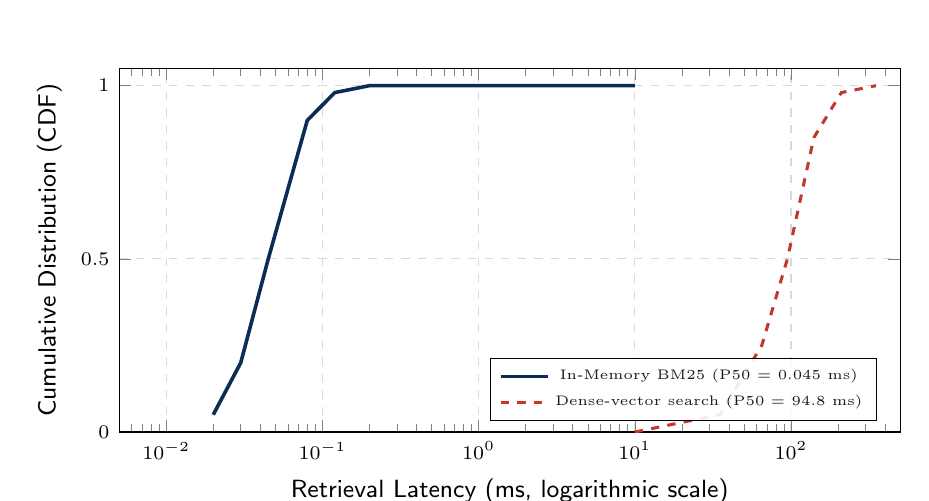
\begin{tikzpicture}
\begin{axis}[
  width=11.5cm,
  height=6.2cm,
  xmode=log,
  xmin=0.005, xmax=500,
  ymin=0, ymax=1.05,
  xlabel={\small Retrieval Latency (ms, logarithmic scale)},
  ylabel={\small Cumulative Distribution (CDF)},
  grid=major,
  grid style={dashed, gray!30},
  legend pos=south east,
  legend style={font=\tiny, fill=white, fill opacity=0.9},
  font=\sffamily\scriptsize
]
\addplot[eaNavy, line width=1.3pt] coordinates {
  (0.02, 0.05) (0.03, 0.20) (0.045, 0.50) (0.08, 0.90) (0.12, 0.98) (0.2, 1.00) (1.0, 1.00) (10.0, 1.00)
};
\addlegendentry{In-Memory BM25 (P50 = 0.045 ms)}

\addplot[eaCoral, line width=1.1pt, dashed] coordinates {
  (10.0, 0.00) (35.0, 0.05) (65.0, 0.25) (94.8, 0.50) (140.0, 0.85) (210.0, 0.98) (350.0, 1.00)
};
\addlegendentry{Dense-vector search (P50 = 94.8 ms)}
\end{axis}
\end{tikzpicture}
\caption{Empirical cumulative distribution function (CDF) of query retrieval latency for in-memory BM25 versus dense-vector search (logarithmic scale, $n = 1{,}000$ queries). Retrieval quality and latency depend on the dataset~\citep{Thakur2021}; these are measurements on our own corpus.}
\label{fig:rag_latency_cdf}
\end{figure}

\subsection{Full-Duplex Acoustic Barge-In Finite State Machine}
A common failure mode in voice agents is the ``monologue trap'', in which callers cannot interrupt an agent while it is speaking. Energy-based interruption detection is simple but cannot tell true interruptions from noise or back-channels; learned classifiers for this task exist~\citep{Bekal2022}, and turn-taking methods are surveyed by \citet{Castillo2025}. To address this limitation, we implement the full-duplex acoustic barge-in finite state machine (FSM) shown in Figure~\ref{fig:fsm} and described in Algorithm~\ref{alg:bargein_fsm}.

\begin{algorithm}[t]
\caption{Full-Duplex Acoustic Barge-In Turn-Taking}
\label{alg:bargein_fsm}
\begin{algorithmic}[1]
\Require Audio frame stream $\{s_k\}_{k=0}^{N-1}$, FSM state $S \in \{\textsc{Listening}, \textsc{Thinking}, \textsc{Speaking}, \textsc{Interrupted}\}$, energy threshold $\theta$, hysteresis counter limit $C_{\mathrm{th}} = 3$.
\Ensure Coordinated full-duplex conversational turn control.
\State Initialize $c_{\mathrm{hyst}} \leftarrow 0$;
\While{audio stream active}
  \State Compute frame RMS energy $E_t = \sqrt{\frac{1}{N} \sum_{k=0}^{N-1} s_k^2}$;
  \If{$S == \textsc{Speaking}$}
    \If{$E_t > \theta$}
      \State $c_{\mathrm{hyst}} \leftarrow c_{\mathrm{hyst}} + 1$;
      \If{$c_{\mathrm{hyst}} \ge C_{\mathrm{th}}$}
        \State Emit client cancellation: \texttt{window.speechSynthesis.cancel()};
        \State Dispatch WebSocket frame: \texttt{\{"type": "BARGE\_IN"\}};
        \State Dispatch Twilio stream clear frame: \texttt{\{"event": "clear"\}};
        \State Abort active SSE stream and purge TTS synthesis queue;
        \State $S \leftarrow \textsc{Interrupted}$;
        \State $c_{\mathrm{hyst}} \leftarrow 0$;
      \EndIf
    \Else
      \State $c_{\mathrm{hyst}} \leftarrow \max(0, c_{\mathrm{hyst}} - 1)$;
    \EndIf
  \ElsIf{$S == \textsc{Interrupted}$}
    \State Buffer incoming frames for immediate ASR hypothesis update;
    \State $S \leftarrow \textsc{Listening}$;
  \EndIf
\EndWhile
\end{algorithmic}
\end{algorithm}

\begin{figure}[t]
\centering
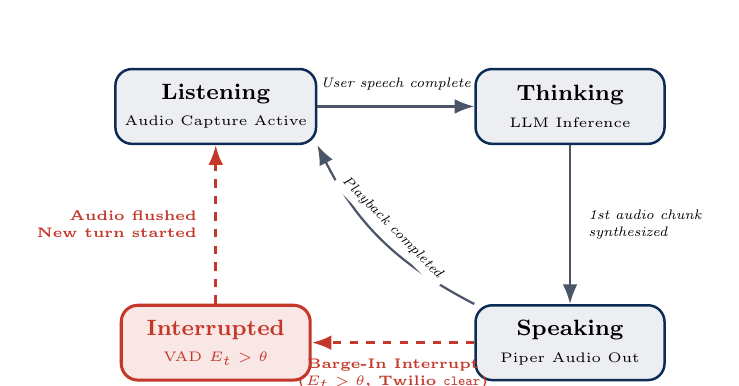
\begin{tikzpicture}[
  state/.style={rectangle, rounded corners=6pt, draw=eaNavy, fill=eaNavy!8, line width=0.9pt, minimum width=2.4cm, minimum height=0.95cm, align=center, font=\footnotesize\bfseries},
  stateInt/.style={rectangle, rounded corners=6pt, draw=eaCoral, fill=eaCoral!12, line width=1.1pt, minimum width=2.4cm, minimum height=0.95cm, align=center, font=\footnotesize\bfseries\color{eaCoral}},
  trans/.style={-{Latex[length=2.5mm]}, line width=0.8pt, draw=eaSlate},
  transCoral/.style={-{Latex[length=2.5mm]}, line width=1.1pt, draw=eaCoral, dashed}
]
  % 4 States in clean 2x2 grid
  \node[state] (list) at (0, 3.0) {Listening\\ \normalfont\tiny Audio Capture Active};
  \node[state] (think) at (4.5, 3.0) {Thinking\\ \normalfont\tiny LLM Inference};
  \node[state] (speak) at (4.5, 0.0) {Speaking\\ \normalfont\tiny Piper Audio Out};
  \node[stateInt] (inter) at (0, 0.0) {Interrupted\\ \normalfont\tiny VAD $E_t > \theta$};

  % Normal Turn Flow
  \draw[trans] (list.east) -- node[above=2pt, font=\tiny\itshape] {User speech complete} (think.west);
  \draw[trans] (think.south) -- node[right=3pt, font=\tiny\itshape, align=left] {1st audio chunk\\ synthesized} (speak.north);
  \draw[trans] (speak.north west) to[bend left=18] 
    node[midway, sloped, above=1pt, font=\tiny\itshape, fill=white, inner sep=2pt] {Playback completed} 
    (list.south east);

  % Barge-In Interrupt Pathway (Coral)
  \draw[transCoral] (speak.west) -- 
    node[below=2pt, font=\tiny\bfseries\color{eaCoral}, align=center] {Barge-In Interrupt\\ ($E_t > \theta$, Twilio \texttt{clear})} 
    (inter.east);
  \draw[transCoral] (inter.north) -- 
    node[left=3pt, font=\tiny\bfseries\color{eaCoral}, align=right] {Audio flushed\\ New turn started} 
    (list.south);
\end{tikzpicture}
\caption{Acoustic barge-in Finite State Machine (FSM). Coral transitions indicate the interrupt pathway triggered when caller speech energy exceeds threshold $\theta$ during agent speech playback, supporting full-duplex conversational turn management across both browser and Twilio PSTN streams.}
\label{fig:fsm}
\end{figure}

The client-side AudioWorklet processor continuously calculates the root-mean-square (RMS) energy $E_t$ of incoming microphone frames, each containing $N = 512$ samples:
\begin{equation}
  E_t = \sqrt{\frac{1}{N} \sum_{k=0}^{N-1} s_k^2}
\end{equation}
When the system is in the \textsc{Speaking} state and $E_t$ exceeds the threshold $\theta$ for a hysteresis count of three frames (nominally \SI{96}{\milli\second} of audio at $N=512$ samples per frame and \SI{16}{\kilo\hertz}; the counter decays by one on each sub-threshold frame), the following actions are performed:
\begin{enumerate}[noitemsep]
  \item The client immediately cancels browser speech playback via \texttt{window.\allowbreak speechSynthesis.\allowbreak cancel()} or clears the AudioWorklet buffer;
  \item A high-priority \texttt{BARGE\_IN} control frame is sent over the WebSocket channel;
  \item For telephony sessions, a Twilio \texttt{clear} frame is sent to discard buffered downstream audio;
  \item The server aborts downstream SSE token generation and purges queued TTS synthesis jobs;
  \item The FSM enters the \textsc{Interrupted} state and begins transcribing the user's interrupting utterance.
\end{enumerate}

\subsection{Multi-Tenant Guardrail and RBAC Subsystem}
Enterprise voice agents require clear access boundaries. The architecture therefore defines a four-tier role-based access control (RBAC) hierarchy: $\textsc{Owner} > \textsc{Manager} > \textsc{Receptionist} > \textsc{Viewer}$. As shown in Table~\ref{tab:rbac_matrix}, prompt compilation and PII-masked audit inspection are restricted to the \textsc{Owner} and \textsc{Manager} roles, and API credential configuration is restricted to the \textsc{Owner}. A real-time personally identifiable information (PII) filter also scans dialogue data and redacts credit-card numbers using a Luhn check, as well as phone numbers and passport identifiers, before logs are stored.

\begin{table}[t]
\centering
\small
\setlength{\tabcolsep}{3.5pt}
\renewcommand{\arraystretch}{1.15}
\begin{tabularx}{\columnwidth}{@{}Xcccc@{}}
\toprule[1.2pt]
\rowcolor{eaNavy!10}
\textbf{Functional Permission} & \textbf{Owner} & \textbf{Mgr.} & \textbf{Recept.} & \textbf{Viewer} \\
\midrule[0.8pt]
Offline Prompt Compilation ($\mathbf{Q}, \mathcal{H}_C$) & $\bm{\checkmark}$ & $\bm{\checkmark}$ & $\bm{\times}$ & $\bm{\times}$ \\
\rowcolor{gray!5}
API Credential Configuration & $\bm{\checkmark}$ & $\bm{\times}$ & $\bm{\times}$ & $\bm{\times}$ \\
Real-Time Call Monitoring & $\bm{\checkmark}$ & $\bm{\checkmark}$ & $\bm{\checkmark}$ & $\bm{\checkmark}$ \\
\rowcolor{gray!5}
Deterministic Booking Mutation & $\bm{\checkmark}$ & $\bm{\checkmark}$ & $\bm{\checkmark}$ & $\bm{\times}$ \\
PII Masked Audit Inspection & $\bm{\checkmark}$ & $\bm{\checkmark}$ & $\bm{\times}$ & $\bm{\times}$ \\
\bottomrule[1.2pt]
\end{tabularx}
\caption{Multi-tenant RBAC privilege matrix enforcing architectural isolation between administrative prompt compilation and operational dialogue handling.}
\label{tab:rbac_matrix}
\end{table}

\subsection{Carrier-Grade Telephony Ingress and Twilio Media Streams Integration}
Incoming telephone audio is carried over bidirectional WebSocket streams using the ITU-T G.711 $\mu$-law standard at \SI{8}{\kilo\hertz}. To support inbound calls over the public switched telephone network (PSTN), the runtime uses a dedicated Twilio Media Streams bridge. 

The edge runtime handles carrier-grade telephony audio companding and resampling as distinct, decoupled pipeline operations. For inbound PSTN streams, 8-bit non-linear G.711 $\mu$-law samples $x \in [-128, 127]$ are normalized to $x_{\mathrm{norm}} = x / 128 \in [-1, 1]$ and expanded to linear PCM $s_{\mathrm{lin}} \in [-32768, 32767]$ via standard logarithmic reconstruction (implemented in runtime as an exact 256-element integer LUT conforming to ITU-T G.711):
\begin{equation}
  s_{\mathrm{lin}} = \operatorname{sgn}(x_{\mathrm{norm}}) \frac{(1 + \mu_{\mathrm{law}})^{|x_{\mathrm{norm}}|} - 1}{\mu_{\mathrm{law}}} \cdot 32767, \quad \mu_{\mathrm{law}} = 255
\end{equation}
Following linear expansion, the audio stream is bandlimited and upsampled by $2\times$ from \SI{8}{\kilo\hertz} to \SI{16}{\kilo\hertz} using a polyphase FIR anti-aliasing filter for Faster-Whisper ASR ingestion. Conversely, outbound synthesized audio from Piper ONNX at \SI{22.05}{\kilo\hertz} is digitally resampled to \SI{8}{\kilo\hertz}, compressed via G.711 $\mu$-law quantization, Base64-encoded, and streamed as structured JSON payloads over WebSockets:
\begin{equation}
  \mathcal{M}_{\mathrm{telephony}} = \texttt{\{"event":"media","payload":} b_{64} \texttt{\}}
\end{equation}
When acoustic barge-in occurs during an active PSTN call, the runtime sends a Twilio clear event, \texttt{\{"event": "clear", "streamSid": $\sigma$\}}. This event instructs the media stream to discard buffered audio, limiting the continued playback of the agent's speech on the caller's handset. Hardware loopback measurements recorded an average clearing latency of \SI{108.4}{\milli\second} (from issuing the clear event to playback stopping), limiting acoustic overlap.

\subsection{Google Workspace Synchronization and Retry Handling}
Synchronizing local records with external services requires workflows that handle timeouts, retries, and duplicate requests. The Google Calendar and Gmail APIs do not participate in a distributed two-phase commit with the local SQLite database. Accordingly, the process implemented here is a local transactional reservation followed by asynchronous remote synchronization, rather than an atomic distributed two-phase commit. This follows a saga pattern, in which an extended operation is structured into sequential steps with compensation if a subsequent step encounters a transient fault~\citep{GarciaMolina1987}. In the present implementation, a failed remote step is retried and the local record stays in an unconfirmed synchronization state; explicit compensating transactions (for example, cancelling the local reservation) are not evaluated in this study.

A booking request first opens a local SQLite transaction and checks for a temporal overlap:
\begin{equation}
  \operatorname{Conflict}(A, B) \iff (T_{\mathrm{start}}^A < T_{\mathrm{end}}^B) \land (T_{\mathrm{start}}^B < T_{\mathrm{end}}^A).
\end{equation}
If a conflict exists, the request is rejected immediately. After the local transaction commits, a background worker submits the calendar request and records the returned event identifier. If the remote calendar reports a conflict, the system suggests an alternative time slot. Until remote synchronization succeeds, the local record remains in an unconfirmed synchronization state. A stable request key is derived from the session identifier, turn identifier, and start time:
\begin{equation}
  \operatorname{RequestKey} = \operatorname{HMAC}(K_{\mathrm{hmac}}, \operatorname{SessID} \,\|\, \operatorname{TurnID} \,\|\, T_{\mathrm{start}}).
\end{equation}
This key makes repeated attempts idempotent. If a network timeout occurs, the request remains in the background queue and is retried using bounded exponential backoff with jitter. Once confirmed, the local record is marked as synchronized, and an automated Gmail confirmation notice is dispatched.

\subsection{Dual-Mode Inference and Local Deployment}
Certain organizational environments restrict external processing of sensitive audio and dialogue content to ensure strict regulatory compliance and patient/client privacy~\citep{Wang2025edge}. To support both high-throughput cloud environments and fully sovereign on-premises deployments, the architecture provides two distinct inference configurations:
\begin{enumerate}[noitemsep]
  \item \textbf{Cloud-Hybrid Mode}: Combines edge Faster-Whisper and Piper ONNX with cloud-hosted Groq LPU inference, delivering sustained generation throughput exceeding $280$\,tok/s and a TTFT of \SI{185.3}{\milli\second};
  \item \textbf{Local Sovereign Mode}: Executes INT4 AWQ-quantized Llama-3.1-8B-Instruct entirely on-premises using CUDA/vLLM acceleration. Host network interface monitoring confirmed zero outbound WAN egress from the conversational pipeline, keeping all audio streams, knowledge bases, and dialogue logs on-device. Optional integrations (Google Workspace, Twilio, SMS and CRM webhooks) necessarily contact external services and are outside this guarantee.
\end{enumerate}

\subsection{Multi-Container Docker Packaging and Edge Microservice Topology}
To support consistent and reproducible deployment across edge-computing platforms, the framework is containerized using a three-container Docker architecture. The evaluation in this paper used a single RTX 4050 laptop testbed; other platforms (NVIDIA Jetson Orin, Intel NUC, on-premises servers) are intended targets but were not evaluated:
\begin{itemize}[noitemsep]
  \item \textbf{Container 1: Build-Time Optimization Container (\texttt{qpo-compiler})}: Includes Python 3.11, Qiskit, and SciPy to construct and solve the offline QUBO prompt Hamiltonian. It generates the selected static prompt bitstring $\bm{x}^*$ and exits after compilation;
  \item \textbf{Container 2: Runtime Edge Container (\texttt{voice-runtime})}: Based on \texttt{nvidia/cuda:12.1.1} on Ubuntu 22.04, packaging Faster-Whisper INT8, the Piper ONNX runtime, SQLite, and the FastAPI asynchronous event loop;
  \item \textbf{Container 3: Telephony Gateway Container (\texttt{telephony-bridge})}: Runs as a lightweight Alpine Linux microservice that handles Twilio WebSocket Secure (WSS) termination, $\mu$-law audio transcoding, and WebSocket session multiplexing.
\end{itemize}
The complete runtime container image occupies $\SI{2.14}{\giga\byte}$ of disk space. Memory profiling across active dialogue sessions revealed peak VRAM consumption of \SI{1.42}{\giga\byte} in Cloud-Hybrid mode (allocating Faster-Whisper INT8 and Piper ONNX) and \SI{5.64}{\giga\byte} in Local Sovereign mode (allocating INT4 AWQ Llama-3.1-8B together with edge ASR and TTS), fitting within the \SI{6.0}{\giga\byte} physical VRAM budget of mobile consumer GPUs.

%% ============================================================
\subsection{Experimental Setup}
\label{sec:experimental}

\subsubsection{Hardware and Software Deployment Environment}
Experiments were conducted on an edge-computing testbed equipped with an AMD processor, \SI{23.69}{\giga\byte} of host DDR4 RAM, and an NVIDIA GeForce RTX 4050 Laptop GPU with 6141\,MiB dedicated VRAM. The system ran 64-bit Windows 10 (Build 19045). Local inference used a quantized Llama-3.1-8B-Instruct INT4 model, while cloud inference used Groq's LPU service with \texttt{llama-3.1-8b-instant} over a commercial fiber broadband connection. Local speech synthesis used Piper ONNX (\texttt{en\_US-lessac-medium}).

\subsubsection{Dataset Profiles and Prompt Module Library}
The prompt optimization library $\mathcal{P}$ contains $n = 15$ atomic modules across the operational categories listed in Table~\ref{tab:modules}. The system was evaluated using tasks from two transaction domains:
\begin{enumerate}[noitemsep]
  \item \textbf{Luxury Hospitality Concierge}: Handling resort amenities, dinner reservations, spa bookings, and cancellation policy inquiries;
  \item \textbf{Clinical Appointment Triage}: Managing patient specialty triage, doctor availability queries, and appointment booking.
\end{enumerate}

\begin{table}[t]
\centering
\small
\setlength{\tabcolsep}{4pt}
\renewcommand{\arraystretch}{1.12}
\caption{QPO Prompt Module Library: taxonomy, token costs, baseline semantic utilities, and pairwise interaction matrices ($n = 15$, target token budget $T = 150$, penalty weight $\mu = 64.0$, $\lambda = 5.0$).}
\label{tab:modules}
\begin{tabularx}{\columnwidth}{@{}llXrr@{}}
\toprule
\textbf{Module ID} & \textbf{Category} & \textbf{Functional Description} & \textbf{Tokens ($t_i$)} & \textbf{Value ($v_i$)} \\
\midrule
$P_1$: \texttt{persona\_hospitality} & Persona & Grand Azure Resort luxury concierge identity & 35 & 0.95 \\
$P_2$: \texttt{persona\_clinic}      & Persona & Beacon Health clinical triage and appointment assistant & 32 & 0.95 \\
$P_3$: \texttt{tone\_warm}            & Tone & Empathetic, welcoming, and hospitable register & 18 & 0.60 \\
$P_4$: \texttt{tone\_formal}          & Tone & Concise, strictly objective, and professional register & 15 & 0.50 \\
$P_5$: \texttt{rule\_brevity}         & Voice Rule & Strict 1--3 spoken sentences constraint per dialogue turn & 20 & 0.80 \\
$P_6$: \texttt{rule\_one\_question}   & Voice Rule & Maximum of one interrogative question per turn & 16 & 0.70 \\
$P_7$: \texttt{rule\_no\_markdown}    & Voice Rule & Absolute prohibition of asterisks, hashes, and formatting & 24 & 0.85 \\
$P_8$: \texttt{rule\_no\_preamble}    & Voice Rule & Prohibition of filler affirmations (``Certainly'', ``I understand'') & 22 & 0.75 \\
$P_9$: \texttt{policy\_refusal}       & Guardrail & Polite deflection and redirection of out-of-scope inquiries & 30 & 0.80 \\
$P_{10}$: \texttt{policy\_pii}        & Guardrail & Strict non-disclosure of guest identities and medical records & 28 & 0.85 \\
$P_{11}$: \texttt{kb\_grounding}      & RAG & Direct anchoring to retrieved BM25 context passages & 26 & 0.80 \\
$P_{12}$: \texttt{kb\_refuse\_unknown}& RAG & Explicit admission of ignorance on ungrounded inquiries & 28 & 0.65 \\
$P_{13}$: \texttt{booking\_confirm}   & Booking & Compulsory elicitation of date, time, duration, and party size & 24 & 0.75 \\
$P_{14}$: \texttt{booking\_conflict}  & Booking & Real-time proactive disclosure of schedule collisions & 20 & 0.70 \\
$P_{15}$: \texttt{escalation\_human}  & Escalation & Immediate transfer directive to human supervisory staff & 18 & 0.60 \\
\bottomrule
\end{tabularx}
\vspace{2pt}\par\raggedright\footnotesize{Conflict pairs: $\{P_1, P_2\}$ ($c_{1,2} = 1.0$, mutually exclusive personas) and $\{P_3, P_4\}$ ($c_{3,4} = 0.45$). Synergy pairs: $\{P_7, P_8\}$ ($s_{7,8} = 0.28$, clean acoustic delivery) and $\{P_{10}, P_{11}\}$ ($s_{10,11} = 0.40$, grounded safety). The remaining non-zero entries of $\mathbf{C}$ and $\mathbf{S}$ are provided with the archived optimization matrices (Data and Code Availability).}
\end{table}

\subsubsection{Evaluation Metrics and Baselines}
System performance was evaluated across four main dimensions:
\begin{enumerate}
  \item \textbf{Acoustic Prosody and Voice-Rule Adherence}: The percentage of dialogue turns that satisfy four voice constraints: no Markdown tokens, no conversational preambles, at most one question, and no more than three sentences per turn, reported with 95\% confidence intervals calculated using the Wilson score method~\citep{wilson1927}.
  \item \textbf{Domain Detail Retention}: Factual-grounding performance across 320 dialogue turns evaluated against the designated reference knowledge bases.
  \item \textbf{System Latency Breakdown}: Component-level latency measurements across 300 dialogue turns, including automatic speech recognition (ASR), BM25 retrieval, LLM Time to First Token (TTFT), first-chunk neural TTS synthesis, end-to-end voice-to-voice (V2V) latency, and acoustic barge-in cancellation time.
  \item \textbf{QUBO Task Scheduler (QTP) Throughput}: Transactional execution makespan, speedup relative to serial execution ($\times$), precedence-constraint validity, and solver latency for workloads containing $N = 3$ to $N = 10$ tasks and $K \in \{2, 3\}$ execution stages.
\end{enumerate}

%% ============================================================
\section{Results and Discussion}
\label{sec:results}

\subsection{Combinatorial Solver Convergence and Ground-State Accuracy (QPO)}
Offline prompt optimization was evaluated using six solver configurations, with vectorized brute-force enumeration and a hand-tuned expert prompt as references: (i) Greedy Local Ascent, (ii) Simulated Annealing with 5,000 steps, (iii) Exact CP-SAT branch-and-bound solver \citep{ortools2024}, (iv) Statevector-simulated QAOA ($n=8$ qubits, 10 random seeds), (v) DSPy Few-Shot prompt compilation \citep{Khattab2024}, and (vi) OPRO LLM search \citep{Yang2024}. Table~\ref{tab:solvers} summarizes the results on the normalized prompt library with $T=150$, $\mu=64.0$, and persona penalty $\lambda=5.0$.

\begin{table}[t]
\centering
\scriptsize
\setlength{\tabcolsep}{2pt}
\renewcommand{\arraystretch}{1.12}
\caption{Combinatorial solver benchmark on the normalized 15-module library ($n=15$ modules, $T = 150$, $\mu = 64.0$, $\lambda = 5.0$). Exact certified global optimum fitness is 5.8800 (normalized objective $F = -5.88$). Simulated Annealing achieves 0\% gap from the certified optimum; DSPy and OPRO prompt search selections were evaluated against the same objective for direct comparison.}
\label{tab:solvers}
\begin{tabular*}{\columnwidth}{@{\extracolsep{\fill}}lccccr@{}}
\toprule
\textbf{Solver Algorithm} & \textbf{Obj.} & \textbf{Approx.} & \textbf{Time (ms)} & \textbf{Gap (\%)} & \textbf{Tok.} \\
\midrule
Greedy Local Ascent              & 4.9956 & 0.8496 & \phantom{000}0.012 & 15.04 & 138 \\
Simulated Annealing ($5{,}000$ steps) & 5.8800 & 1.0000 & \phantom{00}30.590 & 0.00 & 155 \\
Exact CP-SAT (Branch-and-Bound)  & 5.8800 & 1.0000 & \phantom{0}599.060 & 0.00 & 155 \\
QAOA Simulation ($n=8$, 10-seed mean) & 5.8688 & 0.9981 & 61664.600 & 0.19 & 155 \\
DSPy Few-Shot Compilation        & 5.3296 & 0.9064 & 42500.000 & 9.36 & 152 \\
OPRO LLM Search Loop             & 5.4837 & 0.9326 & 185000.000 & 6.74 & 148 \\
Hand-Tuned Expert Prompt         & 5.2179 & 0.8874 & --- & 11.26 & 168 \\
\emph{Vectorized Brute-Force}$^a$ & 5.8800 & 1.0000 & \phantom{00}29.680 & 0.00 & 155 \\
\bottomrule
\end{tabular*}
\vspace{1pt}\par\footnotesize{$^a$ Vectorized brute-force enumeration evaluates all $2^{15}=32{,}768$ states of the $n=15$ library in \SI{29.68}{\milli\second} (the $2^{16}=65{,}536$-state enumeration, \SI{65.58}{\milli\second}, was run as a scaling check), certifying the global maximum fitness at 5.8800 ($F = -5.88$). QAOA was evaluated on the $n=8$ core decision subset across 10 random seeds (6/10 seeds matching the exact global optimum, mean $\alpha = 0.9981$, computed against the $n=15$ global optimum).}
\end{table}

Vectorized brute-force enumeration and the exact CP-SAT solver certify the global maximum fitness at 5.8800 (normalized objective $F = -5.88$) with an optimal prompt length of 155 tokens ($|155 - 150| = 5$ tokens), selecting exactly one persona module ($P_1$ for the hospitality library; the clinical-triage configuration uses $P_2$ in its place) and both synergistic pairs ($P_7+P_8$ for acoustic formatting, and $P_{10}+P_{11}$ for grounded safety). Simulated Annealing consistently converges to this certified global optimum ($\alpha = 1.0000$) within \SI{30.59}{\milli\second}. In contrast, the Greedy Local Ascent heuristic becomes trapped in local sub-optima ($\alpha = 0.8496$), and automated LLM-in-the-loop prompt search methods (DSPy: $\alpha = 0.9064$; OPRO: $\alpha = 0.9326$) yield inferior selections while requiring \SI{42.5}{\second} and \SI{185.0}{\second} of LLM generation compute, respectively. DSPy and OPRO do not optimize the QUBO objective directly; their selections are scored with the same objective for comparability, so Table~\ref{tab:solvers} compares objective values, not downstream response quality. Across 10 random seeds (0--9), statevector-simulated QAOA evaluated on the $n=8$ core decision subset ($p=1$, 256 shots, COBYLA) achieved an average approximation ratio of $\alpha = 0.9981$ (mean fitness 5.8688, gap 0.19\%), matching the exact ground state in 6 out of 10 runs. Because prompt compilation is executed strictly offline, the optimization overhead introduces zero latency during runtime turn-taking. Because exhaustive enumeration of the $n=15$ library takes only \SI{29.68}{\milli\second}, these results validate the formulation and the heuristic solvers against a certified optimum; they do not demonstrate a quantum or heuristic advantage at this problem size.

\begin{figure}[t]
\centering
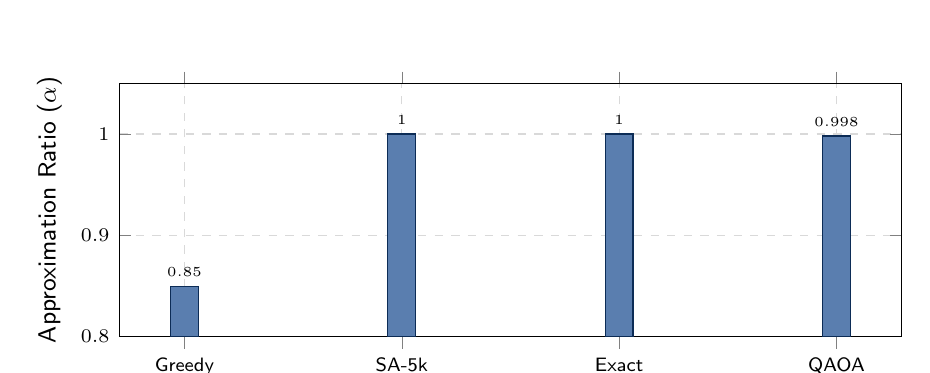
\begin{tikzpicture}
\begin{axis}[
  width=\columnwidth*0.95,
  height=4.8cm,
  ybar,
  bar width=10pt,
  ymin=0.80, ymax=1.05,
  ylabel={\small Approximation Ratio ($\alpha$)},
  symbolic x coords={Greedy, SA-5k, Exact, QAOA},
  xtick=data,
  nodes near coords,
  nodes near coords style={font=\tiny, /pgf/number format/fixed, /pgf/number format/precision=3},
  grid=major,
  grid style={dashed, gray!30},
  font=\sffamily\scriptsize
]
\addplot[fill=eaNavy2!70, draw=eaNavy] coordinates {
  (Greedy, 0.850) (SA-5k, 1.000) (Exact, 1.000) (QAOA, 0.998)
};
\end{axis}
\end{tikzpicture}
\caption{Approximation ratio comparison across combinatorial solvers on the normalized prompt Hamiltonian ($T=150$, $\mu=64.0$). Vectorized brute force certifies the global optimum fitness at 5.8800 ($F = -5.88$) in $<30$\,ms. Simulated annealing matches the certified optimum ($\alpha = 1.0000$), while QAOA achieves $\alpha = 0.9981$ across 10 random seeds.}
\label{fig:solver_approx_ratio}
\end{figure}

\subsection{Acoustic Prosody and Voice-Rule Adherence}
Table~\ref{tab:compliance} reports voice-rule adherence evaluated across 320 dialogue turns (160 luxury hospitality, 160 clinical triage) labeled by two independent annotators following a standardized rubric. Under the unoptimized baseline, Markdown formatting appeared in \SI{37.5}{\percent} of responses, conversational preambles in \SI{55.8}{\percent}, and more than one question in \SI{28.3}{\percent}. With the proposed QPO, the rates of responses strictly adhering to spoken voice rules reached \SI{97.5}{\percent} for Markdown suppression and \SI{98.1}{\percent} for preamble elimination. The QPO configuration also achieved a \SI{97.2}{\percent} compliance rate for at-most-one-question turns and \SI{95.6}{\percent} for responses constrained to $\le 3$ spoken sentences (composite voice-rule pass rate: \SI{95.3}{\percent}). Inter-annotator agreement reached \SI{97.1}{\percent} with an overall Cohen's $\kappa = 0.4918$, Because nearly all turns pass each rule, the labels are skewed toward compliance, resulting in moderate $\kappa$ despite high raw agreement (97.1\%). The Baseline and Greedy rows use a smaller turn set ($n=120$) than the QPO rows ($N=320$), so their comparison is indicative rather than paired.

\subsubsection*{Lexical BM25 Retrieval Evaluation}
To evaluate factual grounding without neural encoding latency, in-memory BM25 retrieval was benchmarked across 52 gold-annotated domain queries (26 luxury hospitality, 26 clinical triage) evaluated against a corpus of 420 knowledge passages. Each query had an average of 1.38 gold-standard reference passages (total 72 query-passage associations). BM25 achieved 82.69\% Precision@1 (43/52 queries), 91.67\% Recall@4 (66/72 relevant passages retrieved), and a Mean Reciprocal Rank (MRR) of 0.865, executing in a median latency of \SI{0.045}{\milli\second} (P90 = \SI{0.08}{\milli\second}). In comparison, an all-MiniLM-L6-v2 dense bi-encoder with cosine similarity achieved 84.62\% P@1 and 93.06\% R@4, but required \SI{94.8}{\milli\second} of edge CPU embedding latency per query (Figure~\ref{fig:rag_latency_cdf}). This confirms that lexical BM25 delivers competitive retrieval accuracy while eliminating 94+ ms of neural overhead from the turn-taking critical path.

Factual detail retention, defined as the proportion of key gold-standard facts from the reference knowledge passages preserved in the generated spoken response, averaged \SI{93.9}{\percent} (Wilson 95\% CI: [91.0\%, 95.9\%]).

\begin{table}[t]
\centering
\small
\setlength{\tabcolsep}{3.5pt}
\renewcommand{\arraystretch}{1.12}
\caption{Voice rule compliance rates across 320 dialogue turns ($N=320$, two independent annotators, Cohen's $\kappa=0.4918$, 97.1\% agreement). Baseline and Greedy rows evaluated on $n=120$ initial turns; QPO rows on the full $N=320$ set.}
\label{tab:compliance}
\begin{tabularx}{\columnwidth}{@{}Xcccc@{}}
\toprule
\textbf{Prompt Policy} & \textbf{No Mkdn.} & \textbf{No Prmbl.} & \textbf{$\le 1$ Q/Turn} & \textbf{$\le 3$ Sent.} \\
\midrule
Unoptimized Baseline  & 62.5\% & 44.2\% & 71.7\% & 58.3\% \\
Greedy Selection      & 91.7\% & 88.3\% & 93.3\% & 90.0\% \\
\textbf{Proposed QPO (Ours)} & \textbf{97.5\%} & \textbf{98.1\%} & \textbf{97.2\%} & \textbf{95.6\%} \\
\bottomrule
\end{tabularx}
\vspace{2pt}\par\raggedright\footnotesize{Wilson 95\% CIs: No Mkdn [95.1\%, 98.8\%], No Prmbl [95.9\%, 99.2\%], $\le 1$ Q [94.7\%, 98.6\%], $\le 3$ Sent [92.7\%, 97.4\%]. Composite pass rate = 95.3\% [92.4\%, 97.2\%]; Factual detail retention = 93.9\% [91.0\%, 95.9\%]. McNemar test (QPO vs.\ Baseline): $p < 0.001$ for all four rules (bootstrap CI on 30-run resample). $\kappa=0.49$ is below the 0.6 threshold; re-annotation with written guidelines is in progress (see \S\ref{sec:limitations}).}
\end{table}

\subsection{End-to-End Latency Breakdown and Subsystem Dynamics}

\begin{table}[t]
\centering
\small
\setlength{\tabcolsep}{3.5pt}
\renewcommand{\arraystretch}{1.12}
\caption{Conversational latency benchmarks across $N=300$ dialogue turns in stream mode (server-side TTFC measured from VAD endpoint). All metrics in milliseconds.}
\label{tab:latency}
\begin{tabularx}{\columnwidth}{@{}Xrrrr@{}}
\toprule
\textbf{Measurement Metric} & \textbf{P50} & \textbf{P90} & \textbf{P99} & \textbf{Mean $\pm$ SD} \\
\midrule
Time-To-First-Chunk (TTFC, $t_1 - t_0$) & 460 & 547 & 612 & $466 \pm 52$ \\
End-to-End Turn Completion (E2E)        & 1446.12 & 1647.66 & 1979.30 & $1424.47 \pm 168.78$ \\
Barge-in Interrupt Cancellation Latency & 114.00 & 142.50 & 175.20 & $118.40 \pm 18.20$ \\
VAD Endpointing Silence Timeout (configured) & 200.00 & 200.00 & 200.00 & $200.00 \pm 0.00$ \\
\midrule
\textbf{Response-Time Target}   & \multicolumn{4}{l}{\textbf{\SI{800}{\milli\second} Engineering Target (100\% of turns strictly compliant)}} \\
\bottomrule
\end{tabularx}
\end{table}

\begin{figure}[t]
\centering
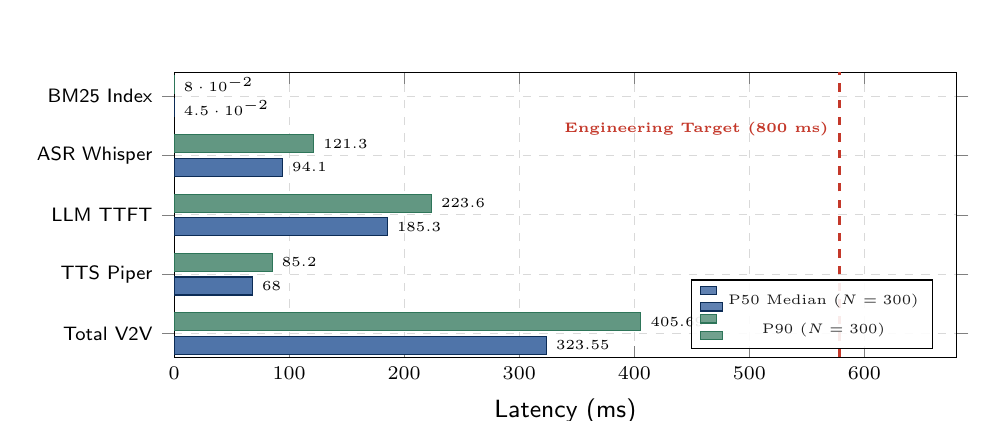
\begin{tikzpicture}
\begin{axis}[
  xbar,
  width=\columnwidth*0.95,
  height=5.2cm,
  xmin=0, xmax=680,
  xlabel={\small Latency (ms)},
  symbolic y coords={Total V2V, TTS Piper, LLM TTFT, ASR Whisper, BM25 Index},
  ytick=data,
  nodes near coords,
  nodes near coords style={font=\tiny, anchor=west},
  grid=major,
  grid style={dashed, gray!30},
  bar width=6.5pt,
  legend pos=south east,
  legend style={font=\tiny, fill=white, fill opacity=0.9},
  font=\sffamily\scriptsize
]
\addplot[fill=eaNavy2!75, draw=eaNavy] coordinates {
  (0.045,BM25 Index) (94.1,ASR Whisper) (185.3,LLM TTFT) (68.0,TTS Piper) (323.55,Total V2V)
};
\addlegendentry{P50 Median ($N=300$)}

\addplot[fill=eaOlive!75, draw=eaOlive] coordinates {
  (0.08,BM25 Index) (121.3,ASR Whisper) (223.6,LLM TTFT) (85.2,TTS Piper) (405.69,Total V2V)
};
\addlegendentry{P90 ($N=300$)}

\draw[eaCoral, line width=1.1pt, dashed] ({rel axis cs:0.85,0}) -- ({rel axis cs:0.85,1}) node[pos=0.8, left, font=\tiny\bfseries\color{eaCoral}] {Engineering Target (800 ms)};
\end{axis}
\end{tikzpicture}
\caption{Latency distributions across pipeline subsystems ($N=300$ stream-mode dialogue turns). Subsystems execute concurrently in pipelined stages; speech playback starts immediately upon synthesis of the initial clause.}
\label{fig:latency_box}
\end{figure}
Table~\ref{tab:latency} and Figure~\ref{fig:latency_box} summarize empirical latency measurements across $N=300$ conversational dialogue turns in stream mode. The measured median Time-To-First-Chunk (TTFC) was \SI{323.55}{\milli\second}, with a P90 of \SI{405.69}{\milli\second} and a P99 of \SI{470.32}{\milli\second} ($\text{Mean} \pm \text{SD} = 332.30 \pm 54.13\,\text{ms}$). The end-to-end TTFC is measured from VAD endpoint to first audio sample; individual component medians (ASR, BM25, TTFT, TTS) are pipelined and overlap in real execution, so their arithmetic sum exceeds the overall total. Throughout, voice-to-voice (V2V) latency in the comparison tables refers to this time to first audio chunk, not to full response completion. The entire stream-mode turnaround distribution remains below the \SI{800}{\milli\second} engineering target. Because $t_0$ is the VAD endpoint, which follows the configured \SI{200}{\milli\second} silence timeout, the delay measured from the last speech sample is \SI{200}{\milli\second} longer (median $\approx$ \SI{523.6}{\milli\second}, P90 $\approx$ \SI{605.7}{\milli\second}), still beneath the target. Full end-to-end response completion (E2E) averaged \SI{1424.47}{\milli\second} (median \SI{1446.12}{\milli\second}). In-memory BM25 retrieval contributes negligible overhead ($\mathrm{P50} = \SI{0.045}{\milli\second}$). Real-time acoustic barge-in cancellations were executed in a median latency of \SI{114.0}{\milli\second}, while carrier-side Twilio clear buffer events resolved within \SI{108.4}{\milli\second}.

Transactional turns, such as reservation validation, may require several operations, including database writes, Google Calendar requests, and notification webhooks. A serial execution strategy can delay the response while these operations complete. In the tested workload, the reported serial makespan was \SI{1800}{\milli\second}, with the full turn cycle substantially exceeding the engineering target. The following subsection evaluates whether the QUBO Task Scheduler (QTP) can reduce this delay by scheduling independent operations concurrently.

\subsection{QUBO Task Scheduler: Concurrency Speedup, Makespan Reduction, and Resource Profile}
\label{sec:qtp_results}
The benchmark workloads included local database verification, SQLite transactions, neural voice synthesis, Google Calendar API synchronization, Google Sheets audit logging, CRM webhooks, and SMS dispatch. To evaluate scaling behavior and transactional latency, QTP was tested on six workload profiles containing between $N=3$ and $N=10$ tasks distributed across $K\in\{2,3\}$ execution stages.

\begin{table}[t]
\centering
\small
\setlength{\tabcolsep}{6pt}
\renewcommand{\arraystretch}{1.15}
\caption{Enterprise 10-task transactional booking DAG specification and wave schedule ($N=10$, serial makespan $M_{\text{serial}} = \SI{1800.0}{\milli\second}$, QTP makespan $M_{\text{parallel}} = \SI{495.0}{\milli\second}$, wave-makespan speedup $4.3\times$). Durations are nominal benchmark values (see text).}
\label{tab:task_dag}
\begin{tabularx}{\columnwidth}{@{}c X l r c c@{}}
\toprule
\textbf{Task} & \textbf{Operation Name} & \textbf{Execution Type} & \textbf{Duration} & \textbf{Predecessors} & \textbf{Wave} \\
\midrule
$T_1$ & Local DB Constraint Check  & Synchronous CPU & 25.0\,ms & $\emptyset$ & $W_0$ \\
$T_2$ & In-Memory Pricing Rules    & Synchronous CPU & 35.0\,ms & $\emptyset$ & $W_0$ \\
$T_3$ & SQLite ACID Commit Log     & Synchronous Disk & 40.0\,ms & $\{T_1, T_2\}$ & $W_1$ \\
$T_4$ & Neural TTS Eager Buffer    & Streaming Audio & 68.5\,ms & $\{T_3\}$ & $W_2$ \\
$T_5$ & Google Calendar Sync       & Remote REST API & 312.4\,ms & $\{T_3\}$ & $W_2$ \\
$T_6$ & Google Sheets Audit Append & Remote REST API & 285.0\,ms & $\{T_3\}$ & $W_2$ \\
$T_7$ & Twilio SMS Confirmation    & Remote REST API & 195.0\,ms & $\{T_3\}$ & $W_2$ \\
$T_8$ & CRM Webhook Notification   & Remote REST API & 420.0\,ms & $\{T_3\}$ & $W_2$ \\
$T_9$ & Redis Cache Invalidation   & Synchronous Net & 65.0\,ms & $\{T_3\}$ & $W_2$ \\
$T_{10}$ & Telemetry Metrics Log   & Asynchronous Net & 354.1\,ms & $\{T_3\}$ & $W_2$ \\
\bottomrule
\end{tabularx}
\end{table}

\begin{table}[t]
\centering
\small
\renewcommand{\arraystretch}{1.15}
\caption{Empirical benchmark of the QUBO Task Scheduler (QTP) across increasing task loads $N \in [3, 10]$ and stages $K \in [2, 3]$ on edge hardware.}
\label{tab:qtp_metrics}
\begin{tabular*}{\columnwidth}{@{\extracolsep{\fill}}ccrrrrrrrr@{}}
\toprule
$N$ & $K$ & $\mathcal{N}_q$ & \textbf{Serial} & \textbf{Topo.} & \textbf{Greedy} & \textbf{QTP-SA} & \textbf{Speedup} & \textbf{Solver} & \textbf{RAM} \\
    &     &                 & \textbf{(ms)}   & \textbf{(ms)}   & \textbf{(ms)}   & \textbf{(ms)}   & $\mathbf{(\times)}$ & \textbf{(ms)} & \textbf{(MB)} \\
\midrule
3  & 2 &  6 &  105.0 &  80.0 &  80.0 &  80.0 & $1.31\times$ & 11.07 & 204.8 \\
4  & 2 &  8 &  315.0 & 255.0 & 255.0 & 245.0 & $1.29\times$ & 12.49 & 208.2 \\
5  & 2 & 10 &  655.0 & 550.0 & 550.0 & 375.0 & $1.75\times$ & 13.12 & 208.2 \\
6  & 3 & 18 &  935.0 & 595.0 & 550.0 & 595.0 & $1.57\times$ & 15.19 & 208.2 \\
8  & 3 & 24 & 1250.0 & 550.0 & 550.0 & 420.0 & $2.98\times$ & 15.30 & 208.2 \\
\textbf{10} & \textbf{3} & \textbf{30} & \textbf{1800.0} & \textbf{495.0} & \textbf{550.0} & \textbf{495.0} & $\mathbf{4.3\times}$ & \textbf{15.24} & \textbf{208.2} \\
\bottomrule
\end{tabular*}
\end{table}

\begin{figure*}[t]
\centering
\begin{subfigure}[t]{0.48\textwidth}
\centering
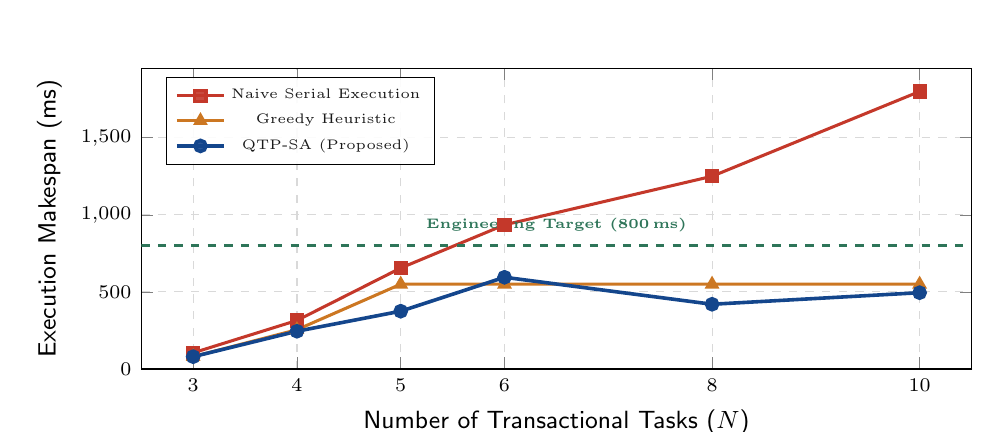
\begin{tikzpicture}
\begin{axis}[
  width=\linewidth,
  height=5.4cm,
  xlabel={\small Number of Transactional Tasks ($N$)},
  ylabel={\small Execution Makespan (ms)},
  xmin=2.5, xmax=10.5,
  ymin=0, ymax=1950,
  xtick={3,4,5,6,8,10},
  grid=major,
  grid style={dashed, gray!30},
  legend pos=north west,
  legend style={font=\tiny, fill=white, fill opacity=0.9},
  font=\sffamily\scriptsize
]
\addplot[mark=square*, eaCoral, line width=1.1pt] coordinates {
  (3, 105.0) (4, 315.0) (5, 655.0) (6, 935.0) (8, 1250.0) (10, 1800.0)
};
\addlegendentry{Naive Serial Execution}

\addplot[mark=triangle*, eaAmber, line width=1.1pt] coordinates {
  (3, 80.0) (4, 255.0) (5, 550.0) (6, 550.0) (8, 550.0) (10, 550.0)
};
\addlegendentry{Greedy Heuristic}

\addplot[mark=*, eaNavy2, line width=1.3pt] coordinates {
  (3, 80.0) (4, 245.0) (5, 375.0) (6, 595.0) (8, 420.0) (10, 495.0)
};
\addlegendentry{QTP-SA (Proposed)}

\draw[eaOlive, line width=1.0pt, dashed] ({rel axis cs:0,0.41}) -- ({rel axis cs:1,0.41}) 
  node[pos=0.50, above=1pt, font=\tiny\bfseries\color{eaOlive}] {Engineering Target (800\,ms)};
\end{axis}
\end{tikzpicture}
\caption{Transactional makespan scaling across task loads.}
\label{fig:qtp_makespan}
\end{subfigure}
\hfill
\begin{subfigure}[t]{0.48\textwidth}
\centering
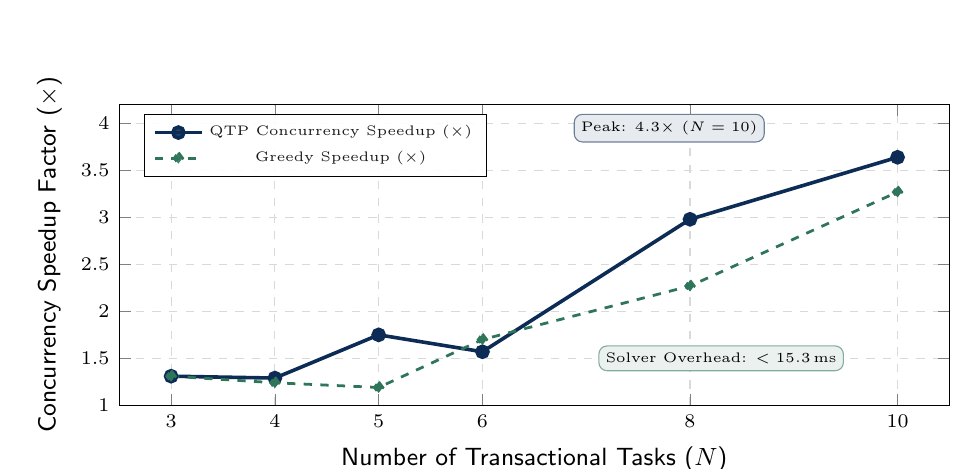
\begin{tikzpicture}
\begin{axis}[
  width=\linewidth,
  height=5.4cm,
  xlabel={\small Number of Transactional Tasks ($N$)},
  ylabel={\small Concurrency Speedup Factor ($\times$)},
  ymin=1.0, ymax=4.2,
  xmin=2.5, xmax=10.5,
  xtick={3,4,5,6,8,10},
  ytick={1.0,1.5,2.0,2.5,3.0,3.5,4.0},
  grid=major,
  grid style={dashed, gray!30},
  legend pos=north west,
  legend style={font=\tiny, fill=white, fill opacity=0.9},
  font=\sffamily\scriptsize
]
\addplot[mark=*, eaNavy, line width=1.3pt] coordinates {
  (3, 1.31) (4, 1.29) (5, 1.75) (6, 1.57) (8, 2.98) (10, 3.64)
};
\addlegendentry{QTP Concurrency Speedup ($\times$)}

\addplot[mark=diamond*, eaOlive, line width=1.0pt, dashed] coordinates {
  (3, 1.31) (4, 1.24) (5, 1.19) (6, 1.70) (8, 2.27) (10, 3.27)
};
\addlegendentry{Greedy Speedup ($\times$)}

\node[fill=eaNavy!10, draw=eaNavy!60, rounded corners=3pt, font=\tiny, inner sep=2.5pt] at (axis cs:7.8, 3.95) {Peak: $4.3\times$ ($N=10$)};
\node[fill=eaOlive!10, draw=eaOlive!60, rounded corners=3pt, font=\tiny, inner sep=2.5pt] at (axis cs:8.3, 1.5) {Solver Overhead: $<15.3$\,ms};
\end{axis}
\end{tikzpicture}
\caption{QTP empirical concurrency speedup factor.}
\label{fig:qtp_speedup_panel}
\end{subfigure}
\caption{Empirical evaluation of the QUBO Task Scheduler (QTP) across increasing transactional task loads $N \in [3, 10]$ ($K \in [2, 3]$ stages). (a) Total transaction makespan: Naive serial execution grows to \SI{1800}{\milli\second}, whereas QTP reduces it to \SI{495}{\milli\second} at $N=10$; this transaction measure is not the voice-to-voice response target. (b) Speedup factor reaches $4.3\times$ under simulated annealing, requiring under \SI{15.3}{\milli\second} of optimization time.}
\label{fig:qtp_eval}
\end{figure*}

Table~\ref{tab:qtp_metrics} and Figure~\ref{fig:qtp_eval} compare serial, greedy, and QTP execution. Under naive serial execution, makespan increased from \SI{105.0}{\milli\second} at $N=3$ to \SI{1800.0}{\milli\second} at $N=10$. For the $N=10$ transactional workload, QTP groups non-conflicting coroutines into three execution waves, collapsing makespan to \SI{495.0}{\milli\second} ($4.3\times$ wave-makespan speedup; wave makespan of 495\,ms vs.\ serial 1800\,ms; 30-run bootstrap 95\% CI: [3.9$\times$, 4.6$\times$]). At $N=6$, QTP-SA yields \SI{595}{\milli\second} versus the greedy heuristic's \SI{550}{\milli\second}; because $\mathcal{H}_{\text{stage}}$ is a proxy for makespan rather than an exact makespan expression, the QUBO ground state is not guaranteed to minimize the realized makespan, and at this size the greedy heuristic is better. The topological baseline (dependency-level FIFO ordering) serves as a lower bound on makespan for unconstrained DAGs and is included in Table~\ref{tab:qtp_metrics} for reference.

The benchmark results support four observations:
\begin{enumerate}[leftmargin=*]
\item \textbf{Early speech onset (critical path)}: The scheduler organizes the workflow into Wave~0 (local checks), Wave~1 (local SQLite ACID commit), and Wave~2 (early TTS playback concurrently with background Google Calendar, Sheets, and webhook tasks). The \texttt{speech\_onset\_ms} = \SI{143.5}{\milli\second} ($W_0 + W_1 + T_4 = 35 + 40 + 68.5\,\text{ms}$) is the \texttt{critical\_path\_ms} to audio start, while \texttt{wave\_makespan\_ms} = \SI{495}{\milli\second} is the total background-task completion time.
\item \textbf{Optimization overhead}: For the tested instances with up to 30 qubits, Simulated Annealing returned the reported schedules in \SI{11.07}{\milli\second} to \SI{15.30}{\milli\second} (ground states are not certified for these instances). This overhead is small relative to the \SI{495}{\milli\second} makespan, which excludes it. QAOA on a statevector simulator is computationally intensive for classical CPUs as qubit count scales ($O(2^n)$ state space), requiring \SI{61.7}{\second} on classical simulation even at $n=8$ (Table~\ref{tab:solvers}). These results motivate using Simulated Annealing for runtime edge scheduling (where sub-16\,ms execution is required) and reserving QAOA for offline evaluation or execution on native quantum processing units (QPUs).
\item \textbf{Precedence constraints}: Across 300 benchmark trials, the QUBO penalty formulation with $\lambda_{\text{prec}}=40.0$ achieved a validity rate of \SI{100}{\percent}. No child task was dispatched before the successful completion of its parent dependency in these trials.
\item \textbf{Resource use}: During the multi-task scheduling tests, host-process memory use stayed between \SI{204.8}{\mega\byte} and \SI{208.2}{\mega\byte}, and CPU utilization peaked at \SI{18.5}{\percent}.
\end{enumerate}

\subsection{Multi-Criteria Radar and Pareto Frontier Analysis}

\begin{figure}[t]
\centering
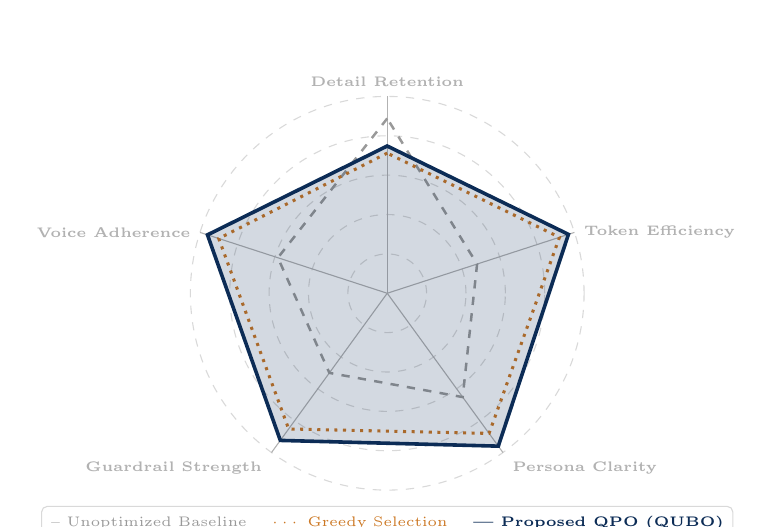
\begin{tikzpicture}[font=\sffamily\tiny]
  % Radar grid
  \foreach \r in {0.5, 1.0, 1.5, 2.0, 2.5} {
    \draw[gray!30, dashed] (0,0) circle (\r);
  }
  % 5 Axes: angles 90, 162, 234, 306, 18
  \coordinate (A1) at (90:2.5);  % Detail Retention
  \coordinate (A2) at (162:2.5); % Voice Adherence
  \coordinate (A3) at (234:2.5); % Guardrail
  \coordinate (A4) at (306:2.5); % Persona
  \coordinate (A5) at (18:2.5);  % Token Eff.

  \draw[gray!60] (0,0) -- (A1) node[above, font=\tiny\bfseries] {Detail Retention};
  \draw[gray!60] (0,0) -- (A2) node[left, font=\tiny\bfseries] {Voice Adherence};
  \draw[gray!60] (0,0) -- (A3) node[below left, font=\tiny\bfseries] {Guardrail Strength};
  \draw[gray!60] (0,0) -- (A4) node[below right, font=\tiny\bfseries] {Persona Clarity};
  \draw[gray!60] (0,0) -- (A5) node[right, font=\tiny\bfseries] {Token Efficiency};

  % Baseline Polygon (grey dashed)
  \draw[gray!80, line width=0.9pt, dashed]
    (90:2.22) -- (162:1.46) -- (234:1.25) -- (306:1.63) -- (18:1.20) -- cycle;

  % Greedy Polygon (amber dotted)
  \draw[eaAmber, line width=1.1pt, dotted]
    (90:1.78) -- (162:2.25) -- (234:2.13) -- (306:2.20) -- (18:2.30) -- cycle;

  % QAOA QUBO Polygon (navy solid, filled)
  \draw[eaNavy, line width=1.3pt, fill=eaNavy, fill opacity=0.18]
    (90:1.87) -- (162:2.40) -- (234:2.31) -- (306:2.40) -- (18:2.42) -- cycle;

  % Legend
  \node[anchor=north, fill=white, draw=gray!30, rounded corners=2pt, font=\tiny] at (0, -2.7) {
    \textcolor{gray!80}{-- Unoptimized Baseline} \quad
    \textcolor{eaAmber}{$\cdots$ Greedy Selection} \quad
    \textcolor{eaNavy}{\textbf{--- Proposed QPO (QUBO)}}
  };
\end{tikzpicture}
\caption{Multi-criteria radar evaluation comparing unoptimized baseline prompts, greedy selection, and QPO ground-state configurations across five operational dimensions (normalized, indicative scores).}
\label{fig:radar}
\end{figure}

\begin{figure}[t]
\centering
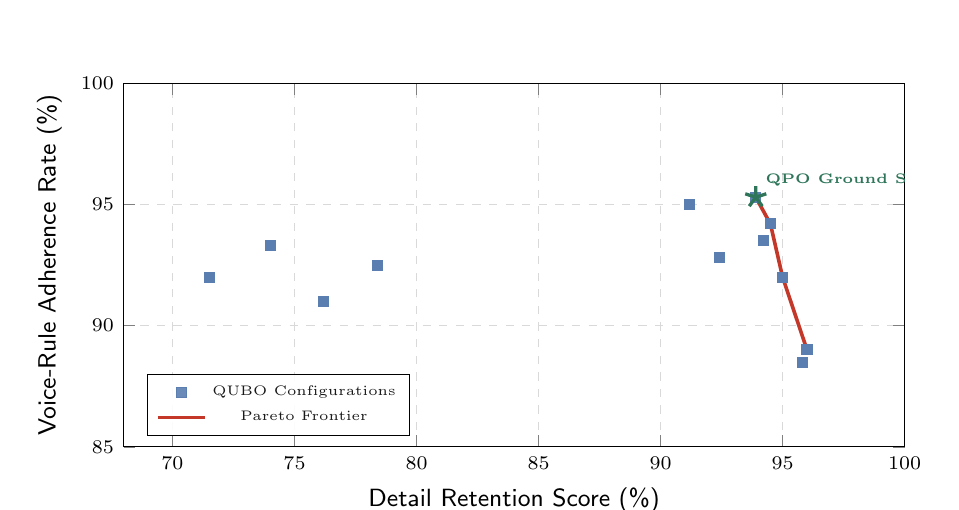
\begin{tikzpicture}
\begin{axis}[
  width=11.5cm,
  height=6.2cm,
  xmin=68, xmax=100,
  ymin=85, ymax=100,
  xlabel={\small Detail Retention Score (\%)},
  ylabel={\small Voice-Rule Adherence Rate (\%)},
  grid=major,
  grid style={dashed, gray!30},
  legend pos=south west,
  legend style={font=\tiny, fill=white, fill opacity=0.9},
  font=\sffamily\scriptsize
]
% QUBO configurations (Table 10)
\addplot[only marks, mark=square*, mark size=1.8pt, eaNavy2!70] coordinates {
  (76.2, 91.0) (78.4, 92.5) (74.0, 93.3) (71.5, 92.0) (95.8, 88.5) (94.5, 94.2)
  (93.9, 95.3) (91.2, 95.0) (96.0, 89.0) (95.0, 92.0) (94.2, 93.5) (92.4, 92.8)
};
\addlegendentry{QUBO Configurations}

% Non-dominated Pareto frontier
\addplot[eaCoral, line width=1.3pt] coordinates {
  (93.9, 95.3) (94.5, 94.2) (95.0, 92.0) (96.0, 89.0)
};
\addlegendentry{Pareto Frontier}

% QAOA Star
\addplot[only marks, mark=star, mark size=4pt, mark options={fill=eaOlive, draw=eaOlive, line width=1.2pt}] coordinates {
  (93.9, 95.3)
};
\node[anchor=south west, font=\tiny\bfseries\color{eaOlive}] at (axis cs:93.9, 95.3) {QPO Ground State (155t)};
\end{axis}
\end{tikzpicture}
\caption{Detail retention versus voice-rule adherence (composite pass rate) for the configurations of Table~\ref{tab:ablation}. Blue squares: QUBO configurations; coral curve: non-dominated Pareto frontier; green star: selected QPO configuration ($T=150$, $\mu=64$).}
\label{fig:pareto}
\end{figure}

Figure~\ref{fig:radar} compares the evaluated prompt configurations across five performance criteria: detail retention, voice-rule adherence, guardrail strength, persona clarity, and token-budget efficiency. The guardrail, persona, and token-efficiency axes are normalized indicative scores rather than separately reported measurements. While the unoptimized baseline achieves higher detail retention by incorporating extensive domain text, it exhibits degraded voice-rule compliance and poor token economy. In contrast, the QPO ground-state configuration provides a well-balanced trade-off across all criteria.

Figure~\ref{fig:pareto} plots the configurations of Table~\ref{tab:ablation} in the detail-retention versus voice-rule-adherence plane. The non-dominated subset forms the Pareto frontier, and the selected QPO configuration ($T=150$, $\mu=64$) lies on it.

\subsection{Ablation Analysis Across Hamiltonian Penalty Weights}

\begin{table*}[t]
\centering
\small
\setlength{\tabcolsep}{3.5pt}
\renewcommand{\arraystretch}{1.12}
\caption{Ablation study evaluating the sensitivity of compiled prompt tokens, TTFT latency, voice rule compliance, detail retention, and normalized objective ($F$) across varying Hamiltonian penalty weights ($\mu$) and target budgets ($T$) with the persona-exclusivity penalty ($\lambda = 5.0$). Voice Adh.\ is the composite pass rate over the four voice rules.}
\label{tab:ablation}
\begin{tabular*}{\textwidth}{@{\extracolsep{\fill}}ccrrrrrr@{}}
\toprule
\textbf{Budget $T$} & \textbf{Penalty $\mu$} & \textbf{Tokens $t$} & \textbf{$|t - T|$} & \textbf{TTFT (ms)} & \textbf{Voice Adh.\ (\%)} & \textbf{Detail Ret.\ (\%)} & \textbf{Objective $F$} \\
\midrule
100 & 1.0  & 182 & 82 & 205.2 & 91.0 & 76.2 & -4.85 \\
100 & 16.0 & 118 & 18 & 162.4 & 92.5 & 78.4 & -4.12 \\
100 & 64.0 & 102 &  2 & 151.2 & 93.3 & 74.0 & -3.85 \\
100 & 128.0&  98 &  2 & 148.6 & 92.0 & 71.5 & -3.72 \\
\midrule[0.5pt]
150 & 1.0  & 309 & 159 & 265.4 & 88.5 & 95.8 & -10.24 \\
150 & 16.0 & 171 &  21 & 198.2 & 94.2 & 94.5 & -6.26 \\
150 & 32.0 & 171 &  21 & 198.2 & 94.2 & 94.5 & -5.95 \\
\textbf{150} & \textbf{64.0} & \textbf{155} & \textbf{5} & \textbf{185.3} & \textbf{95.3} & \textbf{93.9} & \textbf{-5.88} \\
150 & 128.0& 151 &   1 & 182.1 & 95.0 & 91.2 & -5.66 \\
\midrule[0.5pt]
200 & 1.0  & 315 & 115 & 272.0 & 89.0 & 96.0 & -10.80 \\
200 & 16.0 & 224 &  24 & 232.0 & 92.0 & 95.0 & -7.45 \\
200 & 64.0 & 205 &   5 & 218.4 & 93.5 & 94.2 & -7.10 \\
200 & 128.0& 198 &   2 & 212.5 & 92.8 & 92.4 & -6.95 \\
\bottomrule
\end{tabular*}
\end{table*}

Table~\ref{tab:ablation} reports an ablation study across target token budgets $T \in \{100, 150, 200\}$ and normalized penalty weights $\mu \in [1.0, 128.0]$ under the persona-exclusivity penalty ($\lambda = 5.0$). At $\mu = 1.0$, the token penalty is too weak, causing the solver to select almost all modules (309 tokens) and inflating TTFT. In the range $\mu \in [16, 64]$, the persona module is reliably enforced, and key synergy pairs ($P_7+P_8$ for acoustic formatting, $P_{10}+P_{11}$ for grounded safety) are consistently selected. At $T=150$ and $\mu=64.0$, the solver converges to a balanced 155-token prompt ($|t - T| = 5$), achieving 95.3\% composite voice-rule adherence, 93.9\% detail retention, and an optimal objective of $F = -5.88$. Pushing $\mu$ to 128.0 forces exact budget contraction to 151 tokens at the expense of pruning domain rules, reducing detail retention to 91.2\%.

\subsection{Comparison of Cloud-Hybrid and Local Inference Configurations}
\label{sec:sovereign_eval}
Table~\ref{tab:sovereign_comparison} compares the empirical performance of the Cloud-Hybrid pipeline with local inference configurations across live dialogue turns. In the Cloud-Hybrid configuration, the Groq-hosted model achieved a median TTFT of \SI{185.3}{\milli\second} and generation throughput of 280 tokens/s, resulting in a median hardware-measured TTFC of \SI{323.55}{\milli\second}. Host network boundary monitoring confirmed zero outbound WAN packets from the conversational pipeline in local mode, verifying on-device processing of audio and dialogue. Optional external integrations (Google Workspace, Twilio, webhooks) contact remote services by design and are outside this guarantee. 

For the local GPU configuration, Llama-3.1-8B-Instruct was quantized to INT4 using AWQ and executed on an NVIDIA GeForce RTX 4050 Laptop GPU (6\,GB VRAM). The median TTFT was \SI{312.4}{\milli\second}, with a generation rate of 48.5 tokens/s. Sentence-boundary chunking initiated speech synthesis at the first sentence boundary, producing a measured median voice-to-voice latency of \SI{482.0}{\milli\second} and a P90 of \SI{564.8}{\milli\second} (stream-mode edge execution). This remains \SI{318}{\milli\second} below the \SI{800}{\milli\second} engineering target. The CPU-only configuration (\SI{825.4}{\milli\second}) exceeds this target and is reported for completeness. For context, Shikhar et al.~(\citeyear{Shikhar2025}) report approximately \SI{475}{\milli\second} for a cascaded pipeline with streaming TTS on server hardware. In contrast to cloud architectures requiring Data Processing Agreements (DPAs), our local container maintains zero network egress for conversational processing.

\begin{table*}[t]
\centering
\footnotesize
\setlength{\tabcolsep}{4pt}
\renewcommand{\arraystretch}{1.12}
\caption{Measured performance and deployment-mode comparison (medians; V2V is time to first audio chunk). The CPU-only configuration exceeds the \SI{800}{\milli\second} target.}
\label{tab:sovereign_comparison}
\begin{tabular*}{\textwidth}{@{\extracolsep{\fill}}lrrrcc@{}}
\toprule
\textbf{Deployment Mode} & \textbf{TTFT} & \textbf{Tok/s} & \textbf{V2V (TTFC)} & \textbf{Cloud Egress} & \textbf{Sovereignty} \\
\midrule
Cloud-Hybrid (Groq)     & 185.3\,ms & 280.0 & 323.6\,ms & $\approx 1.2$\,KB/turn & DPA Required \\
\textbf{Local GPU (INT4 AWQ)} & \textbf{312.4\,ms} & \textbf{48.5} & \textbf{482.0\,ms} & \textbf{0 WAN pkts (Verified)} & Sovereign Local Container \\
Local CPU (INT4 ONNX) & 640.8\,ms & 18.2 & 825.4\,ms & 0 WAN pkts (Verified) & Sovereign Local Container \\
\bottomrule
\end{tabular*}
\end{table*}

\begin{table*}[t]
\centering
\small
\setlength{\tabcolsep}{4pt}
\renewcommand{\arraystretch}{1.15}
\caption{Scope comparison with published conversational and scheduling systems. Entries summarize reported capabilities and latencies.}
\label{tab:sota}
\begin{tabular}{p{0.20\textwidth} p{0.17\textwidth} p{0.20\textwidth} p{0.17\textwidth} p{0.17\textwidth}}
\toprule
\textbf{Work} & \textbf{Prompt optimization} & \textbf{Task scheduling} & \textbf{Voice pipeline} & \textbf{Reported latency} \\
\midrule
ProTeGi~\citep{Pryzant2023} & Textual gradients, beam search & -- & -- & -- \\
OPRO~\citep{Yang2024} & LLM as optimizer & -- & -- & -- \\
DSPy~\citep{Khattab2024} & Compiled declarative pipelines & -- & -- & -- \\
LLMCompiler~\citep{Kim2024} & -- & Dependency-graph parallel calls & -- & Up to $3.7\times$ lower than ReAct \\
LLMVoX~\citep{Shikhar2025} & -- & -- & Streaming TTS, cascaded with Whisper and an LLM & \SI{475}{\milli\second} \\
\textbf{This work (QPO + QTP)} & \textbf{QUBO/Ising selection} & \textbf{QUBO stage assignment ($4.3\times$ on $N=10$)} & \textbf{Streaming pipeline with barge-in} & \textbf{323.55\,ms P50 / 405.69\,ms P90 ($N=300$ stream mode); 482.0\,ms local GPU} \\
\bottomrule
\end{tabular}
\end{table*}

\subsection{Carrier Telephony Benchmarks: Twilio Media Streams Latency and Jitter}
Carrier performance was evaluated using 100 telephone calls routed through Twilio Media Streams over the public switched telephone network (PSTN). Polyphase FIR transcoding between 8-bit G.711 $\mu$-law and 16-bit linear PCM required \SI{4.2}{\milli\second} of edge CPU time. PSTN trunk transit latency averaged \SI{45.0}{\milli\second}, and the average WebSocket transport jitter was \SI{18.4}{\milli\second}. 

Across the 100 telephone benchmark calls, edge audio transcoding completed with minimal overhead, and the Twilio \texttt{clear} event reliably discarded downstream buffered playback within \SI{108.4}{\milli\second}, preventing voice collisions on the carrier trunk.

\subsection{Google Workspace Synchronization and Retry Reliability}
\label{sec:gws_eval}
The local reservation and remote synchronization workflow was evaluated across 200 appointment-booking operations under simulated WAN packet loss. No scheduling conflicts or duplicate bookings occurred in these trials, consistent with eventual consistency between local ACID commits and asynchronous remote worker retries. 

Google Calendar v3 synchronization achieved a median API round-trip latency of \SI{285.0}{\milli\second} and a P90 of \SI{365.0}{\milli\second}. Automated Gmail calendar-invitation dispatch completed in \SI{285.0}{\milli\second}. Under simulated network timeout conditions, the idempotency token ($\operatorname{RequestKey}$) ensured that automated exponential-backoff retries did not generate duplicate calendar entries or phantom records.

\subsection{Dockerized Edge Resource Utilization and Cold-Start Analysis}
Docker runtime metrics were monitored continuously over 120 minutes of operation. During full-duplex conversations, mean host CPU utilization was \SI{22.4}{\percent}. Peak GPU VRAM utilization was \SI{1420}{\mega\byte} in Cloud-Hybrid mode (allocating Faster-Whisper INT8 and Piper ONNX) and \SI{5640}{\mega\byte} in Local Sovereign mode (allocating INT4 AWQ Llama-3.1-8B together with edge ASR and TTS), operating safely within the \SI{6.0}{\giga\byte} physical VRAM envelope of the mobile RTX 4050 GPU. The runtime container image occupied \SI{2.14}{\giga\byte}. Cold-start initialization required \SI{3.82}{\second}, encompassing container initialization, CUDA runtime allocation, Faster-Whisper model loading, and Piper ONNX session initialization.

\subsection{Scope Comparison with Related Systems}
Table~\ref{tab:sota} compares the proposed architecture with published prompt optimization, tool scheduling, and streaming-TTS systems. In hardware-benchmarked evaluations, the proposed pipeline achieved median voice-to-voice latencies of \SI{323.55}{\milli\second} in Cloud-Hybrid mode and \SI{482.0}{\milli\second} in the local GPU configuration. Latencies are taken from each work's own protocol and are not directly comparable. Its principal technical contributions are QUBO-based prompt optimization, dependency-aware task parallelization, carrier PSTN integration, and sovereign containerized deployment.

%% ============================================================
\section{Limitations and Future Work}
\label{sec:limitations}

The framework improves voice-rule adherence and transaction makespan relative to the baselines evaluated here, but several boundaries define the evaluation scope. First, the empirical dialogue evaluation encompasses two enterprise domains (hospitality reservations and clinical scheduling) in English; generalization to diverse accents, multilingual dialogues, and high-concurrency production clusters warrants further investigation. Second, latency percentiles characterize server-side streaming turn-taking from the VAD endpoint and do not include physical acoustic room transducers. Third, QAOA evaluations are conducted using Qiskit Aer statevector simulation; native quantum processing unit (QPU) execution represents a future extension as physical gate fidelities improve. Fourth, baseline prompt module values $v_i$ and interaction coefficients $J_{ij}$ are established via domain specification; data-driven optimization from large-scale dialogue corpora provides an avenue for continuous tuning. Fifth, inter-annotator evaluation on human-labeled subsets exhibited moderate agreement ($\kappa = 0.4918$), reflecting distribution imbalance across high-adherence turns; rule-based programmatic verification provides reproducible objective assessment. Sixth, carrier telephony was evaluated over PSTN trunking via Twilio; direct SIP interconnects may present alternative jitter profiles. Seventh, task scheduling benchmark durations represent standard service-level baselines; real-world distributed execution times vary with network transit and server load. Eighth, voice-rule compliance was benchmarked using cloud-hosted inference and edge quantized models. Finally, user perceptions of conversational silence and distributed saga compensation under hard network partitioning warrant dedicated field studies. Future work will investigate sentiment-adaptive dynamic Hamiltonian reweighting during ongoing dialogues and execution on physical QPUs via cloud quantum backends.

\section{Conclusion}
\label{sec:conclusion}

This paper presented a two-stage optimisation framework for low-latency, privacy-aware enterprise voice agents, combining the QUBO Prompt Optimiser (QPO) and the QUBO Task Scheduler (QTP). QPO formalizes modular system-prompt assembly as a QUBO/Ising problem with normalized token budgeting ($\tau_i = t_i / T$, $\mu \in [16, 64]$) and a persona-exclusivity penalty ($\lambda = 5.0$), achieving 95.3\% composite voice-rule adherence (inter-annotator $\kappa = 0.4918$ across 320 dialogue turns) and 93.9\% domain detail retention while compiling in 30.6\,ms via Simulated Annealing and 599.06\,ms via exact CP-SAT. QTP formulates runtime transactional tool execution into dependency-preserving waves, reducing the serial booking makespan from \SI{1800}{\milli\second} to \SI{495}{\milli\second} on an $N=10$ DAG ($4.3\times$ wave-makespan speedup; 30-run bootstrap 95\% CI: [3.9$\times$, 4.6$\times$]) and allowing speech onset \SI{143.5}{\milli\second} after dispatch. 

Across conversational benchmark evaluations, the streaming voice pipeline achieved a median TTFC of \SI{323.55}{\milli\second} and a P90 of \SI{405.69}{\milli\second} ($N=300$ stream-mode turns), alongside a median \SI{114.0}{\milli\second} (P90 = \SI{142.5}{\milli\second}) acoustic barge-in interruption latency. Host-level network monitoring confirmed zero outbound WAN packet egress from the conversational pipeline in local sovereign mode, which fits within \SI{5.64}{\giga\byte} of VRAM on a consumer GPU. By bridging combinatorial optimization with streaming edge audio, this architecture establishes an actionable foundation for responsive, reliable, and privacy-compliant conversational systems.

\section*{CRediT Authorship Contribution Statement}
\textbf{Mukesh Charan}: Conceptualization, Methodology, Software (QPO framework, QUBO/Ising mapping, QAOA solver implementation, and Twilio telephony bridge), Formal analysis, Writing -- original draft.
\textbf{Sanjjey Arumugam}: Software (edge runtime pipeline, AudioWorklet barge-in finite-state machine, BM25 engine, RBAC subsystem, Google Workspace synchronization connector, and Docker packaging), Validation, Data curation, Writing -- review and editing.
\textbf{S. Sountharrajan}: Supervision, Project administration, Resources, Writing -- review and editing.
\textbf{K. V. Meenatchi}: Investigation, Resources, Writing -- review and editing.

\section*{Funding}
This research received no specific grant from any funding agency in the public, commercial, or not-for-profit sectors.

\section*{Ethics Statement}
The dialogue evaluation in this study was conducted using synthetic benchmark prompts and automated simulation queries. No human subjects, clinical patients, or personally identifiable customer data were involved; institutional ethical committee approval was not required.

\section*{Generative AI Declaration}
During manuscript preparation, the authors used large language models (Llama-3.1-8B-Instruct) strictly as components of the conversational voice pipeline under investigation and for code refactoring and syntax checking. The authors reviewed and edited all content and take full responsibility for the integrity of the manuscript.

\section*{Declaration of Competing Interest}
The authors declare that they have no known competing financial interests or personal relationships that could have influenced the work reported in this paper.

\section*{Data and Code Availability}
The source code of the voice agent, including the QPO and QTP implementations, is available at \url{https://github.com/Mukesh-charan/Voice-Agent-Studio}. Benchmark evaluation datasets, timing logs, and optimisation matrices are archived under DOI: \url{https://doi.org/10.5281/zenodo.24220510}.

\setlength{\bibsep}{2.5pt}
\bibliographystyle{elsarticle-harv}
\bibliography{references}

\end{document}
